\documentclass[letterpaper]{article} % DO NOT CHANGE THIS
% AAAI-27 Author Kit (official, https://aaai.org/authorkit27/, AuthorKit27.zip, aaai2027.sty dated 2026-10-21).
% AAAI anonymous workshop manuscript.
\usepackage[submission]{aaai2027}  % DO NOT CHANGE THIS
\usepackage[hyphens]{url}  % DO NOT CHANGE THIS
\usepackage{graphicx} % DO NOT CHANGE THIS
\urlstyle{rm} % DO NOT CHANGE THIS
\def\UrlFont{\rm}  % DO NOT CHANGE THIS
\usepackage{natbib}  % DO NOT CHANGE THIS AND DO NOT ADD ANY OPTIONS TO IT
\usepackage{caption} % DO NOT CHANGE THIS AND DO NOT ADD ANY OPTIONS TO IT
\frenchspacing  % DO NOT CHANGE THIS
\usepackage{algorithm}
\usepackage{algorithmic}
\usepackage{booktabs}
\usepackage{array}
\usepackage{amsmath}
\usepackage{placeins} % \FloatBarrier keeps appendix floats in their sections
\pdfinfo{
/TemplateVersion (2027.1)
}
\setcounter{secnumdepth}{2} % Section numbers enabled (permitted by the template: 0, 1 or 2).

\title{BrickForma: Crystallizing LLM Geometric Knowledge\\into Small Models for Text-to-Brick Assembly}
\author{Anonymous submission}
\affiliations{}


% AAAI sets \@maketitle in the full-width first-page title block.
% Append the teaser inside that block so it precedes the two-column abstract.
\AddToHook{cmd/@maketitle/after}{\par
\begingroup
\centering
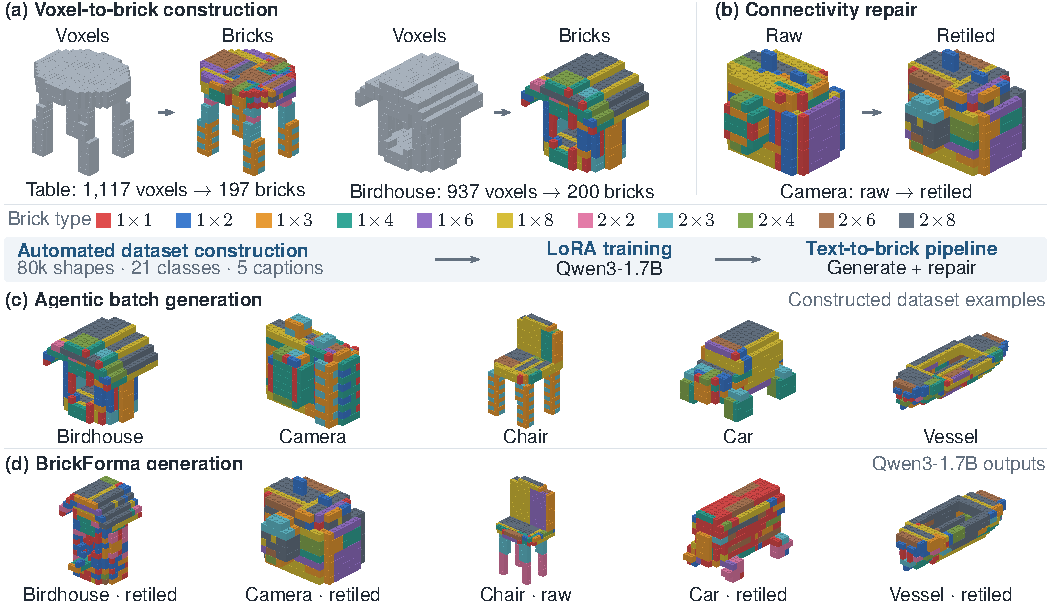
\includegraphics[width=\textwidth]{figure1.pdf}\par
\captionof{figure}{BrickForma overview. (a) Source voxels are tiled with rectangular bricks. (b) Retiling reconnects raw predictions. (c) Brick targets are constructed from LLM-authored voxel generators. (d) Sample outputs of the fine-tuned Qwen3-1.7B pipeline. Colors identify brick sizes, and gray marks source voxels.}
\label{fig:teaser}
\par
\endgroup
}

\begin{document}
\maketitle
\begin{abstract}
Can a language model turn a short description into a three-dimensional assembly? In \textsc{Text-to-Brick}, a generator must infer dimensions and proportions, place discrete pieces, and account for stud connectivity. We present BrickForma, which transfers geometric knowledge from large language models through executable parametric programs. These programs generate 80,000 voxel models in 21 categories on a $48^3$ grid, with five description levels per shape. Same-color tiling, connection analysis, and local repair produce checked brick targets for fine-tuning Qwen3-1.7B. At inference, a mixed-integer program seeks an exact cover of the predicted voxel union with one stud-connected component. On 265 matched prompts, BrickForma's raw outputs attain the highest mean VQAScore (0.1079), PE (0.1572), and SigLIP2 (0.0565) among the three systems. BrickGPT leads VQAScore at the shortest description level and has a lower mean invalid-placement ratio (0.00\% versus 0.81\%). On 110 earlier raw/retiled pairs, the number of single-component layouts rises from 18 to 110, and all pairs have equal occupied voxel unions after translation.
\end{abstract}


\section{Introduction}
Spatial reasoning supports tasks from robotics to automated design. Recent benchmarks use paper folding and procedural drawing to test how large language models (LLMs) infer shapes and transformations~\cite{zhou2026paperfolding,luo2026geogrambench}. Can a model also turn a short description into a three-dimensional object whose pieces are correctly sized, placed, and joined?

A request such as \emph{a simple chair} leaves dimensions, proportions, and part layout implicit. A generator must infer that geometry, discretize it into fixed-size pieces at integer positions, and create stud connections between layers. Pieces can share a side while belonging to separate assemblies. In the \textsc{Text-to-Brick} task, a generator turns a natural-language description into placements that express the requested shape as a single stud-connected assembly.

BrickGPT learns to predict placements autoregressively and uses physics-aware rollback during inference~\cite{brickgpt}. BrickNet encodes assembly connectivity with a graph that supports more part and connection types~\cite{bricknet}. These approaches motivate two questions. \textbf{Q1. How well do generators complete geometry from limited linguistic information?} A comparison by description level reveals behavior on short prompts that an aggregate mean can obscure. \textbf{Q2. How can a compact generator acquire the geometric knowledge needed to fill in missing details?} Large models can describe object proportions and functional parts. Turning that knowledge into checked layouts requires an explicit representation of geometry and connections.

BrickForma uses executable programs to make geometric knowledge available for training (Figure~\ref{fig:teaser}). With GPT-6.1 Sol assistance, we write parametric generators that vary part dimensions, proportions, openings, and support arrangements. The programs produce 80,000 voxel models spanning 21 categories on a $48^3$ grid. Five levels of bilingual descriptions give progressively richer specifications of the same geometry. Same-color tiling, connection analysis, and local repair convert the voxels into checked brick targets. The integrated release records 79,301 models that pass the dataset's geometric checks. English caption--placement pairs supervise a LoRA adaptation of Qwen3-1.7B~\cite{qwen3,lora}.

At inference, the model predicts dimensions and positions as a placement sequence. The sequence supplies a voxel union for geometric reconstruction. For drafts that need repair, mixed-integer linear programming seeks a tiling of that union with one stud-connected component. The solver can therefore change the parts and their connections while retaining the occupied volume.

We evaluate the raw BrickForma outputs against BrickGPT and BrickNet on 265 matched prompts. BrickForma has the highest mean VQAScore, PE, and SigLIP2 in aggregate. At L1, BrickGPT leads VQAScore, and BrickForma leads PE and SigLIP2. An earlier audit of 110 raw/retiled pairs tests occupied-volume preservation and stud connectivity.

\noindent\textbf{Program-based transfer with checked geometry.}
BrickForma converts LLM-authored parametric programs into training layouts for a 1.7B-parameter model. At inference, an exact-cover reconstruction step addresses errors in the predicted brick connections.

\noindent\textbf{A five-level dataset and matched evaluation.}
BrickMore-48 links each source shape to five levels of description. We evaluate three systems at each level and report three measures of rendered text--image alignment, an invalid-placement ratio, and an audit of reconstruction on paired exports.


\begin{figure*}[t]
\centering
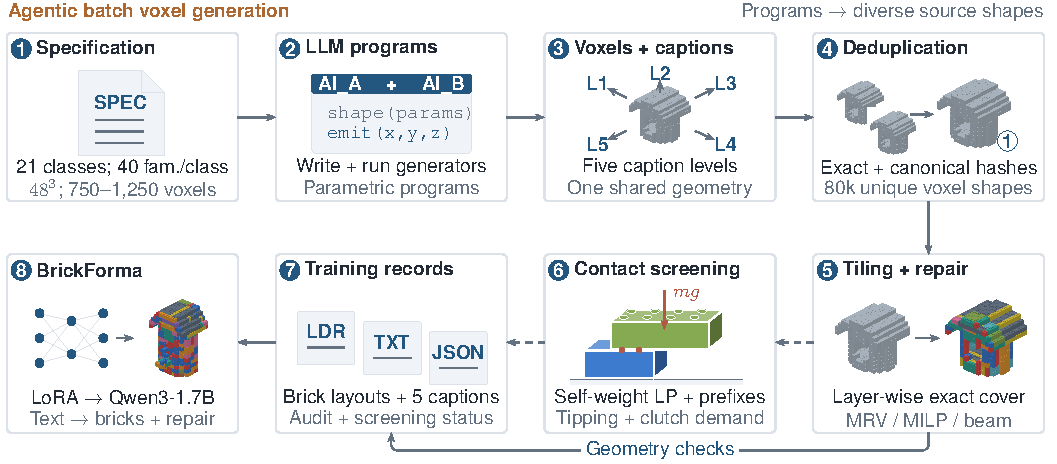
\includegraphics[width=\textwidth]{figure2.pdf}
\caption{Data-construction workflow. GPT-6.1 Sol assists in writing parametric programs that produce voxel shapes and captions. The shapes are deduplicated, tiled, repaired, and checked before export for fine-tuning. Dashed arrows trace contact screening and its recorded status. Brick colors follow the legend in Figure~\ref{fig:teaser}.}
\label{fig:data-workflow}
\end{figure*}

\section{Related Work}
\paragraph{Brick assembly and generation.}
Prior work treats brick assembly as graph generation, sequential construction, or structure understanding~\cite{thompson2020lego,brickbybrick,breakandmake}. BrickGPT predicts autoregressive placement sequences and checks candidate placements during decoding~\cite{brickgpt}. BrickNet represents a wider range of parts and connectors with an assembly graph~\cite{bricknet}. BrickForma generates absolute grid positions for rectangular footprints and reconstructs the predicted volume to enforce stud connectivity.

\paragraph{Stability analysis.}
StableLego uses a force-balance model to assess block-stacking assemblies~\cite{stablelego}. BrickForma checks stud connectivity and voxel coverage during geometric reconstruction. The dataset's contact-based screening makes additional assumptions about forces and ground contact (Appendix~\ref{app:dataset}).

\paragraph{Procedural data and parameter-efficient fine-tuning.}
Procedural generation offers control over shape variation and scale~\cite{infinigen}. BrickForma uses a language model to author executable generators, checks their geometric outputs algorithmically, and fine-tunes a text-only model on the resulting caption--placement pairs using LoRA~\cite{lora}. Its training format follows BrickGPT's serialized placements~\cite{brickgpt}.

\section{Dataset Construction}
\label{sec:dataset}
\subsection{Parametric Voxel Generation}
GPT-6.1 Sol assists in writing parameterized programs for 21 object categories. Each program defines an object family through part dimensions, proportions, openings, and support arrangements. Executing the programs gives 80,000 source voxel models in two 40,000-model shards on a $48^3$ grid, with 750--1,250 occupied cells per object. Exact and canonical occupancy hashes over 48 axis/sign transforms found no cross-shard duplicates. Geometry plans and version identifiers accompany the records (Figure~\ref{fig:data-workflow}).

BrickMore-48 pairs each shape with five bilingual descriptions. L1 expresses the object and its main parts, while progressively richer descriptions add structure, proportions, appearance, and views. The geometry is shared by all five levels, so the same target provides supervision for both concise and detailed requests. Appendix~\ref{app:dataset} gives a birdhouse example.

\subsection{Voxel-to-Brick Conversion and Checks}
The conversion tiles each layer with same-color rectangular footprints and inspects the resulting stud components. Local bridging and retiling address ungrounded components, with edits recorded against the source voxels. The retile release raises the geometry-pass count from 65,503 to 79,298, recovering 13,795 failures. Across the corpus it adds 228,582 and removes 125 voxels, and 31,532 passing models require no edits.

The release checks that the target voxels are six-neighbor connected, every brick component is grounded, and brick placement exactly covers the derived target. Several individually grounded brick components may pass these release checks. Inference uses a stricter single-component constraint. Contact-based gravity screening records a separate outcome (Appendix~\ref{app:dataset}).

\subsection{Integrated Release and Training Corpus}
The full retile release contains 702 geometry failures. A revised batch-B piano release passes all 1,905 slots where the full retile release passed 1,902, giving a report-derived integrated count of $79{,}298-1{,}902+1{,}905=79{,}301$. Table~\ref{tab:training-data} reports the release and recorded fine-tuning counts.
\begin{table}[t]
\centering
\small
\setlength{\tabcolsep}{4pt}
\begin{tabular}{lr}
\toprule
\multicolumn{2}{l}{\emph{Dataset (release reports)}} \\
\midrule
Source models / categories / grid & 80,000 / 21 / $48^3$ \\
Bilingual caption records & 400,000 \\
Failing in full retile release & 702 (0.88\%) \\
Passing in full retile release & 79,298 \\
Piano models restored by revised release & 3 \\
Integrated passing models & 79,301 \\
\midrule
\multicolumn{2}{l}{\emph{Fine-tuning corpus}} \\
\midrule
(model, English caption) samples & 396,610 \\ % Training manifest confirmation pending
Training / validation samples & 356,955 / 39,655 \\
Tokens over 3 epochs & 2,228,044,818 \\ % Training manifest confirmation pending
\bottomrule
\end{tabular}
\caption{Dataset and fine-tuning corpus. The two blocks are counted separately: the upper block from the dataset release reports, the lower block as recorded for the fine-tuning run.}
\label{tab:training-data}
\end{table}


\section{BrickForma Text-to-Brick Model}
\label{sec:model}
\subsection{Fine-Tuning}
\label{sec:training}
We fine-tune Qwen3-1.7B with LoRA on English L1--L5 captions and their checked brick layouts. A model-level 9:1 split keeps descriptions of the same shape together. The $48^3$ grid uses 20 oriented footprints (11 brick sizes up to planar rotation). The instruction lists the allowed dimensions, and the target gives one placement per line, such as $2{\times}4\ (x,y,z)$. Dimensions are serialized Y-first, then X. The sequence describes geometry and omits color.

Fine-tuning follows the BrickGPT Qwen3 script~\cite{brickgpt} (Table~\ref{tab:finetune-config}). Unpacked sequences preserve caption boundaries. The run reached 133,860 steps in 25.3 hours on eight GPUs. Validation loss reached 0.0308 at step 79,000, the released checkpoint, and 0.0339 at the end of epoch 3. Appendix~\ref{app:training} records the validation checkpoints.
\begin{table}[t]
\centering
\small
\setlength{\tabcolsep}{3pt}
\begin{tabular}{@{}l>{\raggedright\arraybackslash}p{0.58\linewidth}@{}}
\toprule
Item & Value \\
\midrule
Base model & Qwen3-1.7B (bf16) \\
Adaptation & LoRA, $r=16$, $\alpha=32$, dropout $0.05$, all linear layers \\
Optimization & LR $10^{-4}$, cosine, 100 warm-up steps, 3 epochs \\
Batch / max length & effective 8 (8 GPUs $\times$ 1) / 8,192 \\
Hardware & DDP, 8$\times$RTX 4090D (24\,GB) \\
Released checkpoint & step 79,000 (best validation loss) \\
Software & transformers 4.51.3, trl 0.17.0, peft 0.15.2 \\
\bottomrule
\end{tabular}
\caption{Fine-tuning configuration (details in Appendix~\ref{app:training}).}
\label{tab:finetune-config}
\end{table}


\subsection{Inference and Retiling}
Algorithm~\ref{alg:inference-retiling} samples with thinking disabled, temperature $0.7$, top-$p$ $0.9$, and at most 8,192 new tokens. It tries seeds 42, 104, and 2026, keeping the first completed draft that passes the geometry validator or the completed draft with the fewest format, library, bounds, and overlap errors. A valid draft with a single stud component is returned as is.

For other drafts, the pipeline forms the in-bounds voxel union $C$ of supported placements, counting overlaps once. Mixed-integer linear programming (MILP) seeks an exact cover of $C$ with one stud-connected component at 12, 60, and 180 seconds. An accepted solution passes an independent audit of placement validity, coverage, and connectivity. If the budget is exhausted, the pipeline can retain the draft and queue a new seed. Recovery runs can sample additional seeds or extend the budget to 600 seconds. We call the drafts \emph{raw} and the accepted reconstructions \emph{retiled}.
\begin{algorithm}[tb]
\caption{BrickForma inference and retiling}
\label{alg:inference-retiling}
\small
\begin{algorithmic}[1]
\REQUIRE prompt $c$; fine-tuned model $\theta$; library $\mathcal{L}$ (20 footprints); seeds $S=(42,104,2026)$; MILP tiers $T=(12,60,180)$\,s
\ENSURE $(B_{\mathrm{out}}, \textit{status})$, $\textit{status}\in\{\textsc{Success},\textsc{Draft},\textsc{Failed}\}$
\STATE $B \gets \emptyset$; $A \gets \emptyset$
\FOR{$s \in S$}
  \STATE $(B_s,\textit{rep}) \gets \mathrm{Parse}(\theta.\mathrm{Generate}(c,\ \mathrm{seed}{=}s))$
  \STATE $A \gets A \cup \{(B_s,\textit{rep})\}$
  \IF{$\textit{rep}.\mathrm{complete} \land \textit{rep}.\mathrm{valid}$}
    \STATE $B \gets B_s$; \textbf{break}
  \ENDIF
\ENDFOR
\IF{$B=\emptyset$}
  \IF{no completed draft in $A$}
    \RETURN $(\emptyset,\ \textsc{Failed})$
  \ENDIF
  \STATE $B \gets \arg\min_{\text{completed } a\in A} \mathrm{Err}(a)$
\ENDIF
\IF{$\mathrm{Err}(B)=0 \land \mathrm{StudComponents}(B)=1$}
  \RETURN $(B,\ \textsc{Success})$ \COMMENT{keep a valid connected raw layout}
\ENDIF
\STATE $C \gets \mathrm{UnionVoxels}(B;\ \mathcal{L},\ 48^3)$ \COMMENT{clip; overlaps count once}
\FOR{$\tau \in T$}
  \STATE $B^{*} \gets \mathrm{MILP\text{-}SingleStudCover}(C,\ \tau)$
  \IF{$B^{*}\neq\emptyset \land \mathrm{Audit}(B^{*},C)$}
    \RETURN $(B^{*},\ \textsc{Success})$
  \ENDIF
\ENDFOR
\STATE $\mathrm{QueueReseed}(c)$
\RETURN $(B,\ \textsc{Draft})$ \COMMENT{unsolved: keep raw draft}
\end{algorithmic}
\end{algorithm}


\section{Comparative Evaluation}
\label{sec:eval}
\subsection{Setup and Metrics}
\label{sec:setup}
The November 16 evaluation covers 21 categories and five description levels. The main comparison, Group B, uses 265 shared prompts, with 53 per level and one delivered output per system per prompt. All BrickForma outputs in Group B are raw generations from its Q8\_0 weights. Group A contains 260 matched prompts for BrickGPT and BrickNet. Together the two groups contain 1,315 LDraw exports (Figure~\ref{fig:comparison-cohorts}).

\emph{Text--image alignment.}
Each export is rendered with uniform yellow material in eight $512{\times}512$ orthographic views, at azimuths spaced $45^\circ$ apart and at $25^\circ$ elevation. Each alignment score takes the maximum over views and is then averaged over prompts. VQAScore~\cite{vqascore} uses the first-token probability of \textquotedblleft Yes\textquotedblright\ from Qwen2.5-VL-7B-Instruct~\cite{qwen25vl}. PE~\cite{pe} uses cosine similarity of normalized image and text embeddings, and SigLIP2~\cite{siglip2} uses the sigmoid of the image--text logit.

\emph{Invalid placements.}
For an export with $n$ placements in file order, let $I_i$ indicate whether placement $i$ is invalid given the preceding placements under BrickNet's inset collision kernel~\cite{bricknet}. We compute $P_{\mathrm{inv}}=n^{-1}\sum_{i=1}^{n}I_i$ per export and report its mean across prompts.

\subsection{Main Results}
\begin{table}[t]
\centering\small
\setlength{\tabcolsep}{3pt}
\begin{tabular}{lrrrr}
\toprule
System & $P_{\mathrm{inv}}\downarrow$ & VQAScore $\uparrow$ & PE $\uparrow$ & SigLIP2 $\uparrow$ \\
\midrule
BrickForma & 0.81\% & \textbf{0.1079} & \textbf{0.1572} & \textbf{0.0565} \\
BrickGPT & \textbf{0.00\%} & 0.0926 & 0.1459 & 0.0262 \\
BrickNet & 17.88\% & 0.0259 & 0.1173 & 0.0016 \\
\bottomrule
\end{tabular}
\caption{Group B means on 265 matched prompts. BrickForma uses delivered raw outputs. Bold marks the best mean.}
\label{tab:main}
\end{table}

BrickForma attains the highest mean VQAScore (0.1079), PE (0.1572), and SigLIP2 (0.0565) on Group B (Table~\ref{tab:main}). It exceeds BrickGPT on 188, 166, and 168 of the 265 prompts for these metrics, respectively. The six paired alignment comparisons pass Holm correction under both tests (Appendix~\ref{app:eval}). BrickGPT has the lowest mean $P_{\mathrm{inv}}$ (0.00\%), followed by BrickForma (0.81\%) and BrickNet (17.88\%). Figures~\ref{fig:comparison-means} and~\ref{fig:comparison-distributions} show the means and score distributions.

\subsection{Performance across Description Levels}
\begin{table*}[t]
\centering\small
\setlength{\tabcolsep}{3pt}
\begin{tabular}{lrrlrrrr}
\toprule
Level & $n$ & Words & System & $P_{\mathrm{inv}}\downarrow$ & VQAScore $\uparrow$ & PE $\uparrow$ & SigLIP2 $\uparrow$ \\
\midrule
L1 & 53 & 13.4 & BrickForma & 0.41\% & 0.1841 & \textbf{0.1409} & \textbf{0.0254} \\
 &  &  & BrickGPT & \textbf{0.00\%} & \textbf{0.1911} & 0.1323 & 0.0132 \\
 &  &  & BrickNet & 15.14\% & 0.0445 & 0.1032 & 0.0002 \\
\midrule
L2 & 53 & 26.4 & BrickForma & 0.78\% & \textbf{0.1651} & \textbf{0.1453} & \textbf{0.0241} \\
 &  &  & BrickGPT & \textbf{0.00\%} & 0.1354 & 0.1391 & 0.0206 \\
 &  &  & BrickNet & 17.74\% & 0.0579 & 0.1037 & 0.0013 \\
\midrule
L3 & 53 & 37.3 & BrickForma & 0.73\% & \textbf{0.1467} & \textbf{0.1479} & \textbf{0.0717} \\
 &  &  & BrickGPT & \textbf{0.00\%} & 0.1061 & 0.1396 & 0.0199 \\
 &  &  & BrickNet & 23.30\% & 0.0211 & 0.1075 & 0.0012 \\
\midrule
L4 & 53 & 52.3 & BrickForma & 1.38\% & \textbf{0.0239} & \textbf{0.1792} & \textbf{0.0914} \\
 &  &  & BrickGPT & \textbf{0.00\%} & 0.0198 & 0.1609 & 0.0487 \\
 &  &  & BrickNet & 18.68\% & 0.0023 & 0.1344 & 0.0016 \\
\midrule
L5 & 53 & 78.6 & BrickForma & 0.75\% & \textbf{0.0198} & \textbf{0.1727} & \textbf{0.0698} \\
 &  &  & BrickGPT & \textbf{0.00\%} & 0.0107 & 0.1575 & 0.0286 \\
 &  &  & BrickNet & 14.56\% & 0.0035 & 0.1379 & 0.0035 \\
\bottomrule
\end{tabular}
\caption{Group B means by description level. Each level contains 53 prompts per system. Words is the mean English word count. Bold marks the best mean.}
\label{tab:levels}
\end{table*}

BrickForma leads PE and SigLIP2 at all five levels and VQAScore at L2--L5 (Table~\ref{tab:levels} and Figure~\ref{fig:comparison-levels}). At L1, the prompts average 13.4 words. BrickGPT scores 0.1911 on VQAScore and BrickForma scores 0.1841. BrickGPT has the lowest mean $P_{\mathrm{inv}}$ at each level. Figure~\ref{fig:gallery} shows two L1 and two L2 examples under matched rendering conditions.
\begin{figure*}[t]
\centering
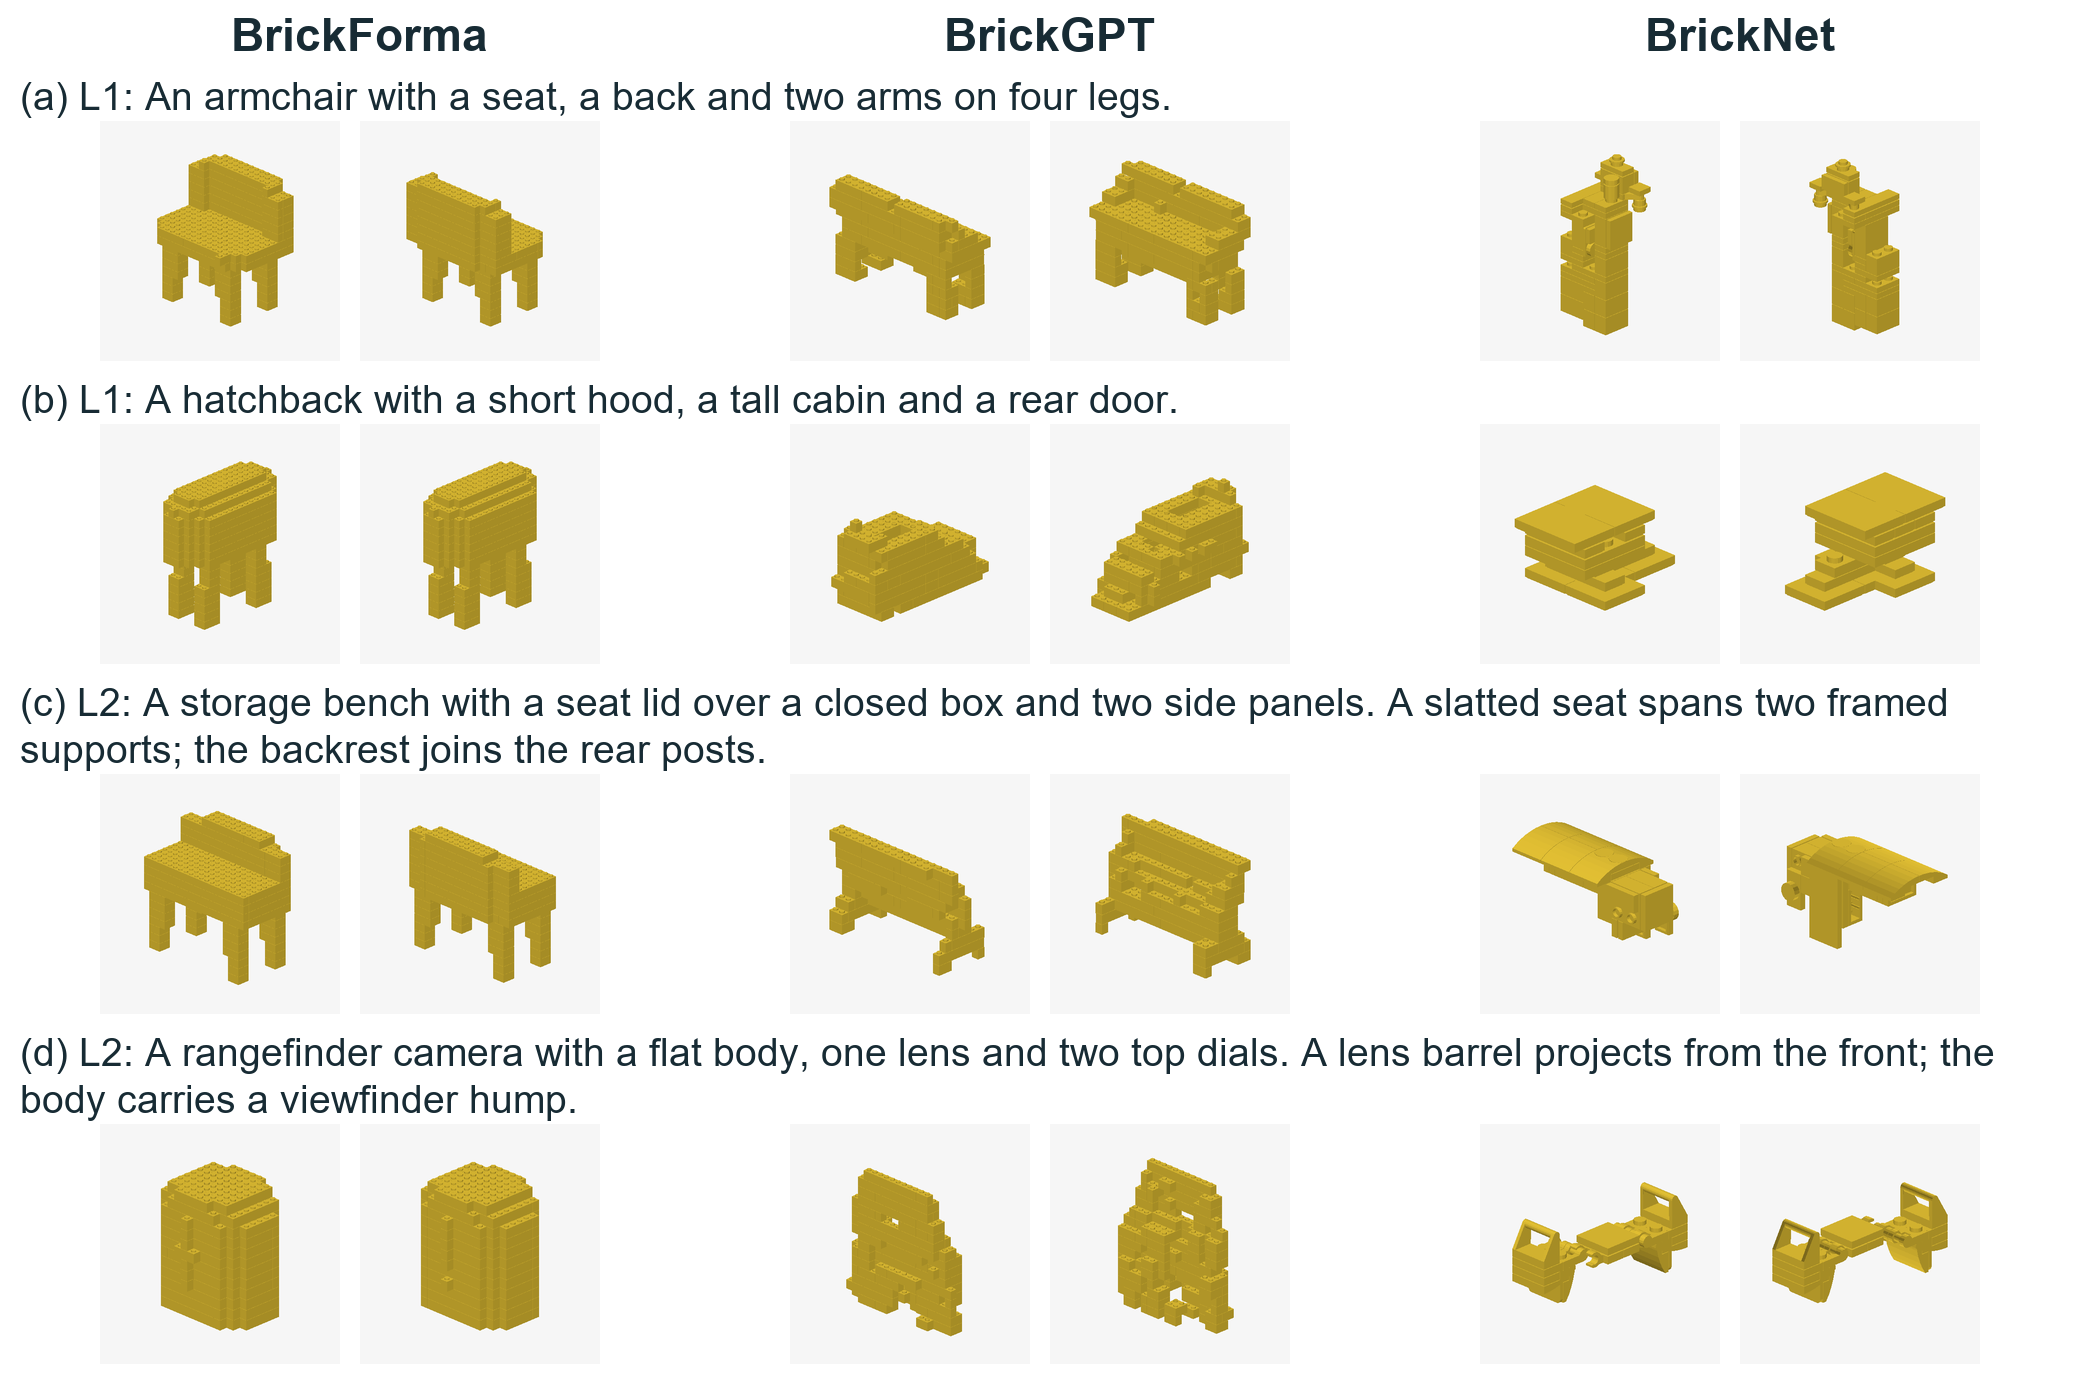
\includegraphics[width=\textwidth]{figures/matched_short_prompts_20261116.png}
\caption{Four matched Group B examples with the same prompts, render settings, and azimuths ($45^\circ$ and $225^\circ$) across systems. The highest VQAScore belongs to BrickForma for the chair and bench, BrickGPT for the hatchback, and BrickNet for the camera.}
\label{fig:gallery}
\end{figure*}


\subsection{Raw versus Retiled Outputs}
\begin{table}[t]
\centering
\small
\begin{tabular}{lrr}
\toprule
Metric & Raw & Retiled \\
\midrule
$P_{\mathrm{inv}}$ $\downarrow$ & 0.1897\% & 0.0000\% \\
VQAScore $\uparrow$ & 0.2065 & 0.2071 \\
PE $\uparrow$ & 0.1858 & 0.1859 \\
SigLIP2 $\uparrow$ & 0.1379 & 0.1261 \\
Mean parts & 178.7 & 421.2 \\
\bottomrule
\end{tabular}
\caption{Earlier repair comparison on 110 pairs sharing the same prompt, model identifier, and caption.}
\label{tab:raw-retiled}
\end{table}

We examine reconstruction on 110 raw/retiled pairs from an earlier 114-prompt comparison (Table~\ref{tab:raw-retiled}). Retiling reduces mean $P_{\mathrm{inv}}$ from 0.1897\% to 0.0000\% and increases mean part count from 178.7 to 421.2. VQAScore and PE change little, while SigLIP2 falls from 0.1379 to 0.1261. Each pair shares a prompt and model identifier.

\subsection{Geometric Reconstruction Audit}
\label{sec:diagnostics}
We define stud contacts by footprint overlap across adjacent layers. We map the same 110 pairs to a grid with 20 LDU horizontal pitch and 24 LDU layer height and translate each export to a common occupied-cell origin. All 110 pairs have equal occupied voxel unions after translation. Single-component layouts rise from 18 to 110, and overlap-free layouts rise from 100 to 110 (Table~\ref{tab:export-audit}).
\begin{table}[t]
\centering\small
\begin{tabular}{@{}lrr@{}}
\toprule
Export measure & Raw & Retiled \\
\midrule
Single stud component & 18/110 & 110/110 \\
Mean stud components & 4.29 & 1.00 \\
No body-cell overlap & 100/110 & 110/110 \\
\midrule
\multicolumn{3}{@{}l@{}}{Equal voxel unions after translation: 110/110} \\
\bottomrule
\end{tabular}
\caption{Earlier export audit of 110 matched raw/retiled pairs. Union equality uses translation normalization.}
\label{tab:export-audit}
\end{table}

In the separate 525-prompt diagnostic run, 46 raw layouts have a single stud component. All 525 final layouts form one component and preserve their corresponding target unions after the reported recovery procedure (Appendix~\ref{app:eval}).

\subsection{Evaluation Boundaries}
The comparison uses delivered exports from systems with different inference settings and part libraries. The description levels vary in both content and length. PE truncates 59 Group B prompts and SigLIP2 truncates 106 (Appendix~\ref{app:eval}). Uniform yellow rendering evaluates shape and layout without assessing color fidelity. The paired reconstruction audit describes the delivered selected pairs. Its denominator excludes unsuccessful solver attempts.

\section{Limitations and Discussion}
The program-based transfer combines generator design, geometric validation, and supervised fine-tuning. Isolating the contribution of large-model authoring would require an alternative generator evaluated under a matched training budget.

The dataset release checks grounding and coverage, and reconstruction enforces a single stud-connected component. Mechanical stability and a feasible assembly order require separate measurements. The integrated release and the training run record their counts separately (Table~\ref{tab:training-data}).

\section{Conclusion}
BrickForma converts program-generated voxels into checked brick layouts and uses them to fine-tune Qwen3-1.7B. Its raw outputs lead the three alignment metrics in aggregate on 265 matched prompts, with a mean invalid-placement ratio of 0.81\%. In the earlier paired audit, exact-cover reconstruction restores stud connectivity while preserving the occupied voxel union.

\bibliography{references}
\FloatBarrier
\appendix
\section{Technical Appendix: Dataset Details}
\label{app:dataset}
The historical figures and tables in this appendix retain the supplied measurements and model renders, with labels translated into English. They use release-specific versions and criteria and are not substitutes for the integrated statistics or the current main comparison.

\emph{Caption example.} The five captions of one model share a prefix and add detail level by level. The L1 prompt is \textquotedblleft An oval birdhouse with curved roof, enclosed room and front entrance.\textquotedblright\ Its L5 description is: ``An oval birdhouse with curved roof, enclosed room and front entrance. The protective roof joins the walls; the circular front entrance reaches a real interior cavity. Curved substantial surfaces carry their continuously attached functional parts. Overall width is 1.15 times depth; height is 0.80 times width. Parts follow functional positions. Continuous red, tan, brown color regions distinguish the body and attachments. The front reveals functional parts; side and top views reveal depth, connections and layout.''

\begin{table}[!htbp]
\centering
\small
\setlength{\tabcolsep}{3pt}
\begin{tabular}{lrrr}
\toprule
Release & Passing & Added & Removed \\
\midrule
Strict v3 & 7,902 & -- & -- \\
Relaxed & 65,503 & 428,278 & 38,230 \\
Local bridging and retiling & 79,298 & 228,582 & 125 \\
\bottomrule
\end{tabular}
\caption{Geometric pass counts of the 80,000 source models under successive conversion releases (relaxed: several grounded components allowed), with total voxels added and removed, as in the corresponding release reports.}
\label{tab:conversion}
\end{table}

\begin{figure*}[!htbp]
\centering
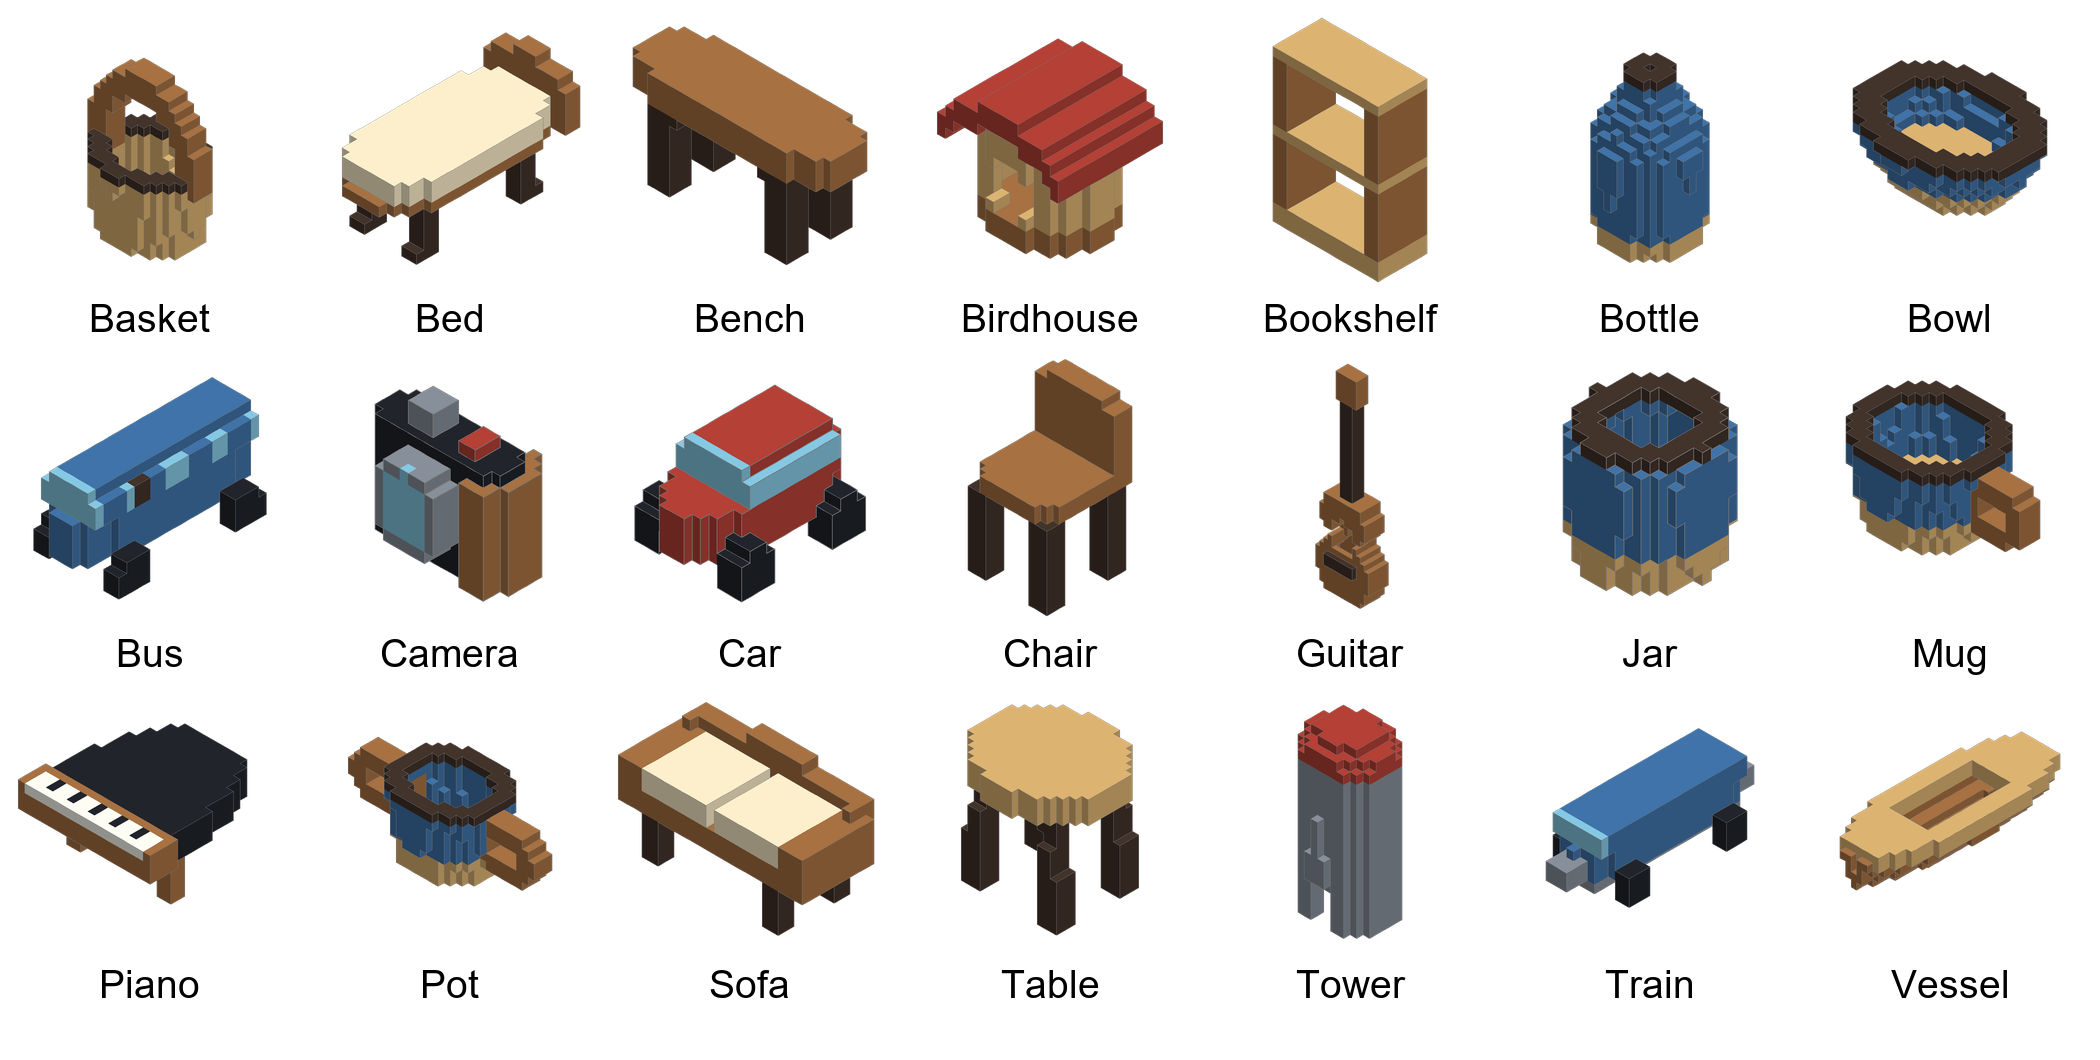
\includegraphics[width=\textwidth]{figures/image7_en.png}
\caption{Voxel model samples spanning the 21 object categories.}
\end{figure*}

\begin{figure*}[t]
\centering
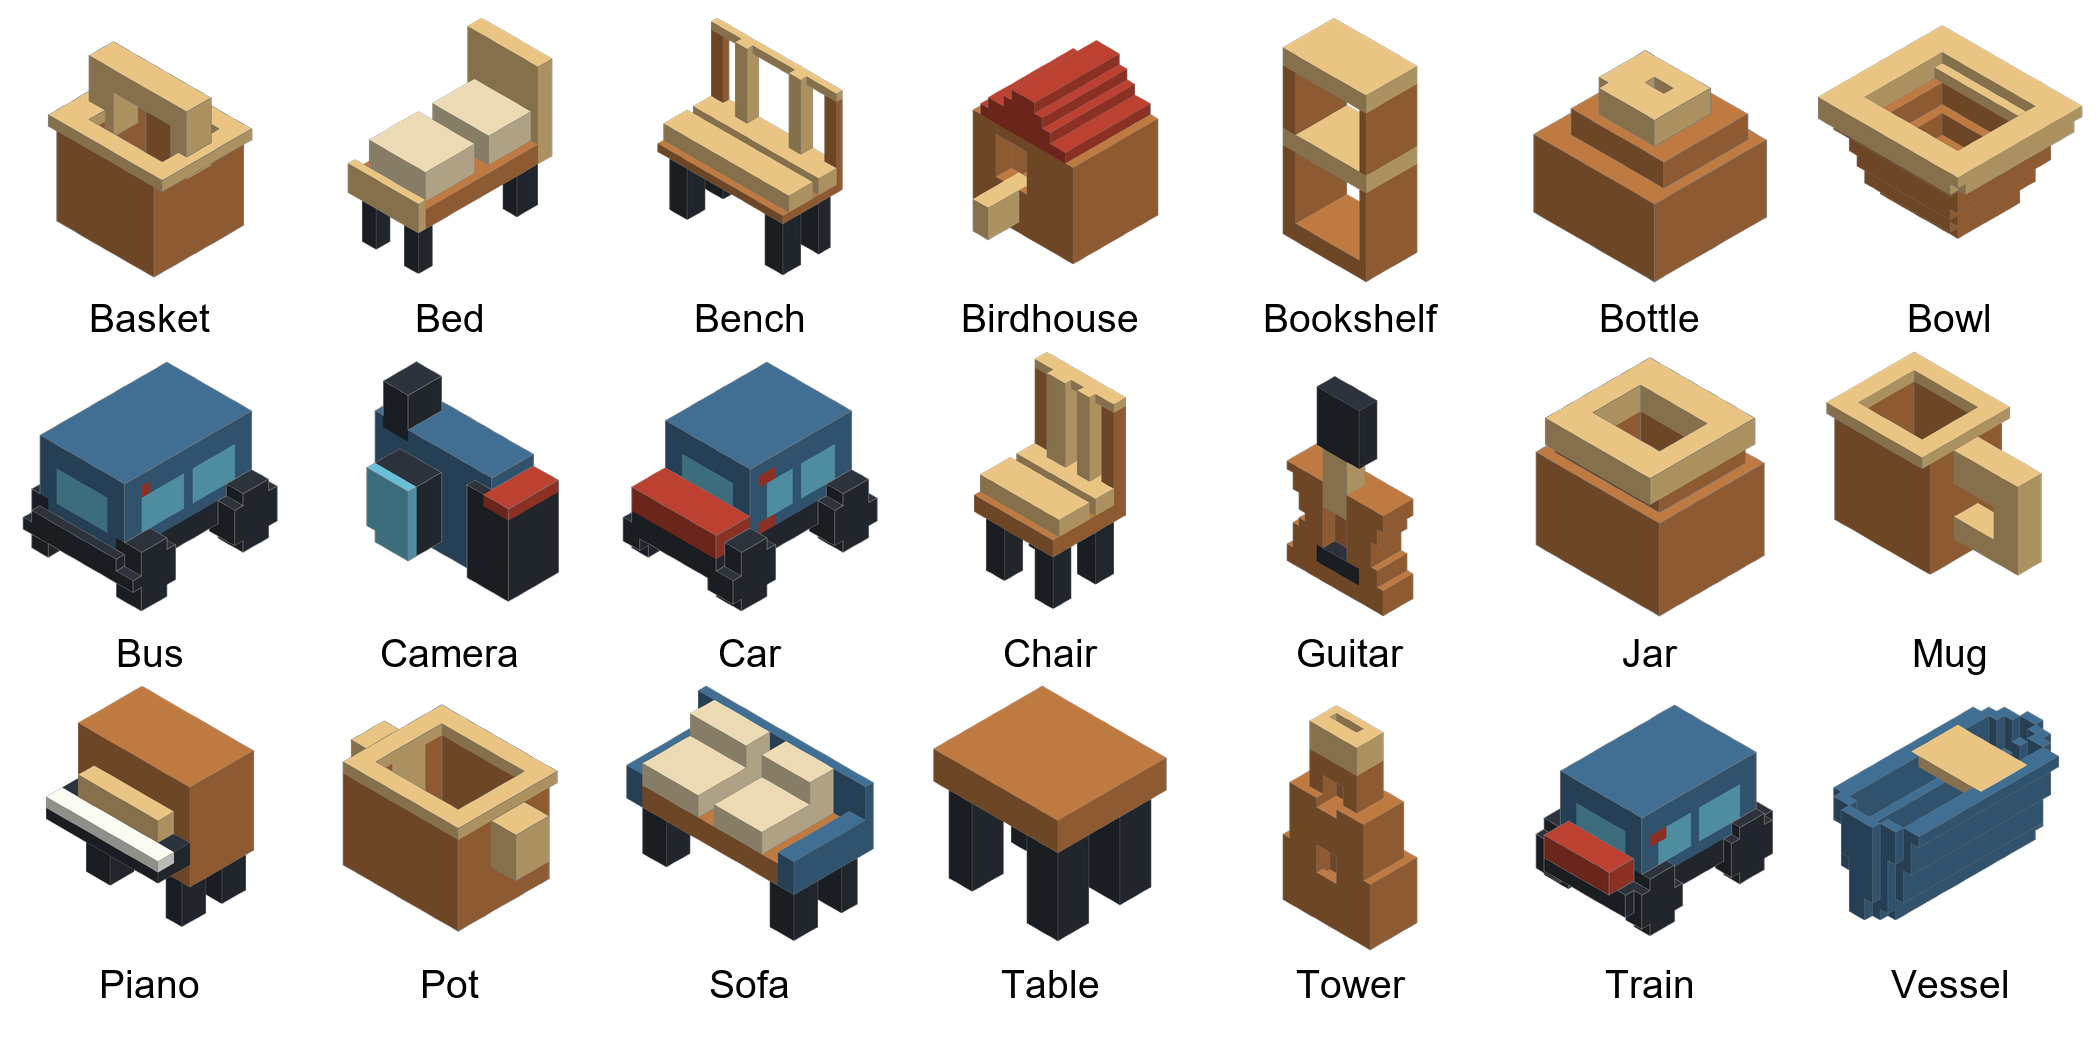
\includegraphics[width=\textwidth]{figures/image8_en.png}
\caption{Additional historical voxel model examples.}
\end{figure*}

\begin{figure*}[!htbp]
\centering
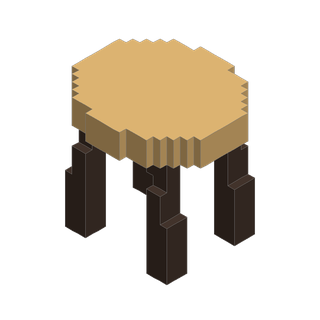
\includegraphics[width=0.118\textwidth]{figures/image4.png}\hfill
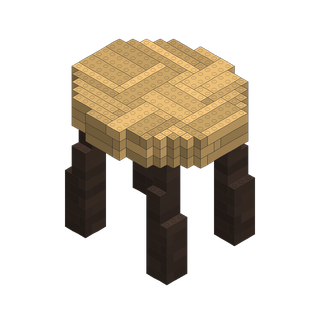
\includegraphics[width=0.118\textwidth]{figures/image5.png}\hfill
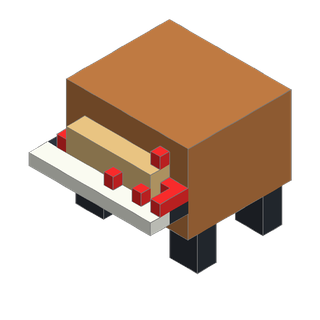
\includegraphics[width=0.118\textwidth]{figures/image2.png}\hfill
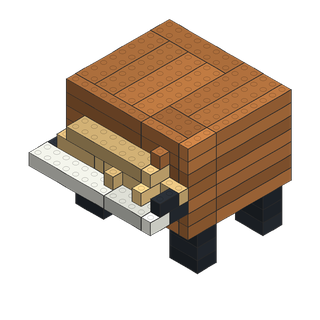
\includegraphics[width=0.118\textwidth]{figures/image3.png}\hfill
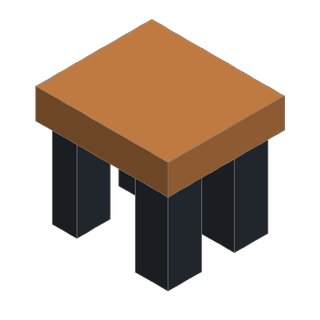
\includegraphics[width=0.118\textwidth]{figures/image9.png}\hfill
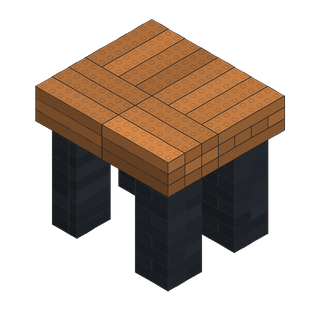
\includegraphics[width=0.118\textwidth]{figures/image10.png}\hfill
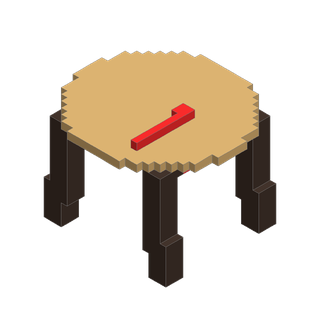
\includegraphics[width=0.118\textwidth]{figures/image11.png}\hfill
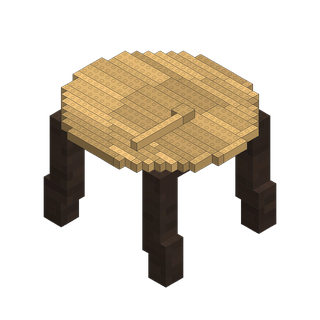
\includegraphics[width=0.118\textwidth]{figures/image12.png}
\caption{Historical examples of voxel targets and brick layouts after local repair.}
\end{figure*}

\begin{figure*}[t]
\centering
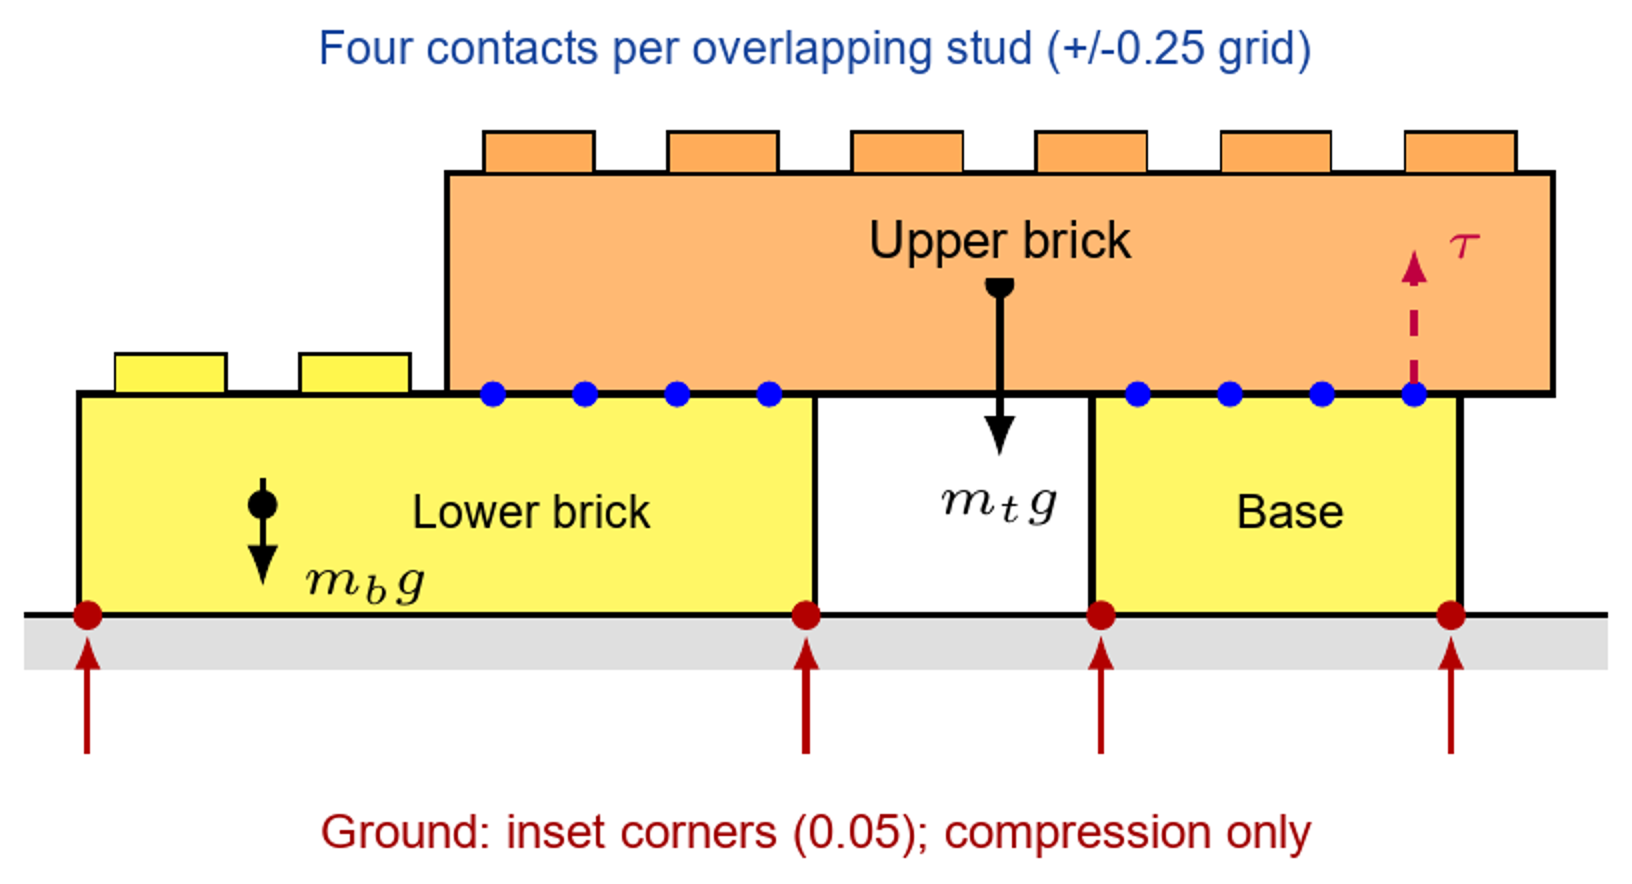
\includegraphics[width=0.75\textwidth]{figures/image13_en.png}
\caption{Historical contact-based gravity screening model, with English labels. The stated contact and ground assumptions are retained.}
\end{figure*}

\begin{figure*}[!htbp]
\centering
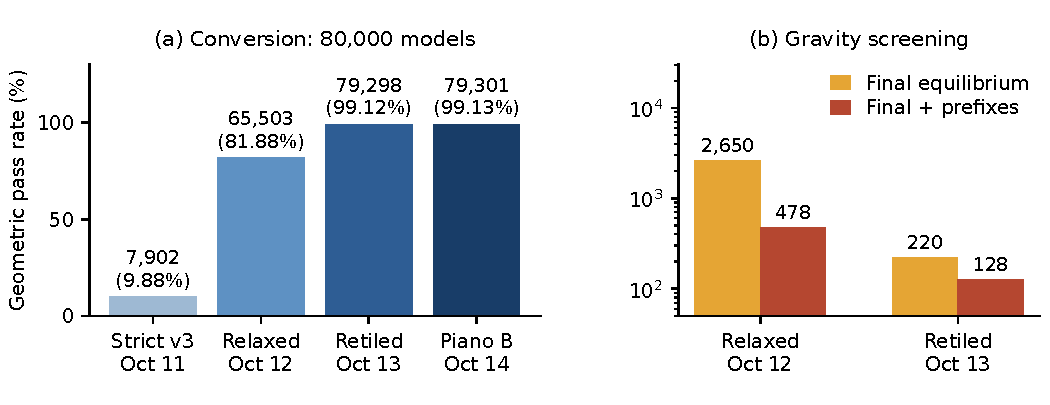
\includegraphics[width=\textwidth]{figures/image14_en.pdf}
\caption{Historical comparison of geometric conversion and screening outcomes across releases; values as in the corresponding release reports (Table~\ref{tab:conversion}).}
\end{figure*}

\begin{figure*}[!htbp]
\centering
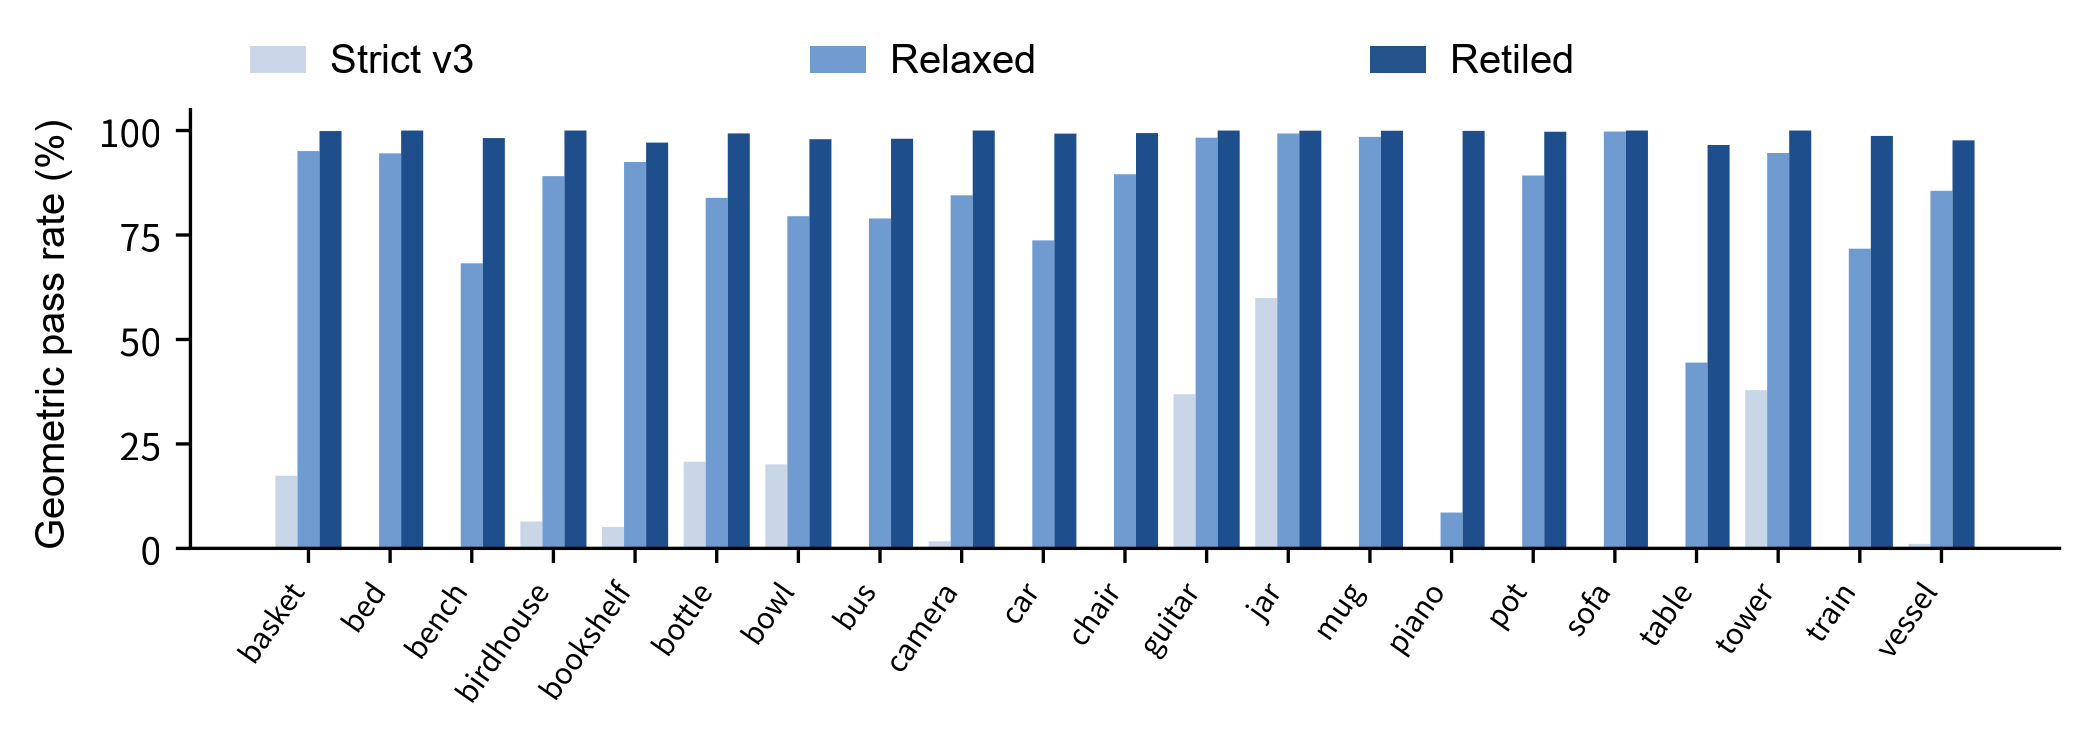
\includegraphics[width=\textwidth]{figures/image15_en.png}
\caption{Historical category-level geometric pass rates. Version and numerical labels require verification.}
\end{figure*}

\begin{figure*}[t]
\centering
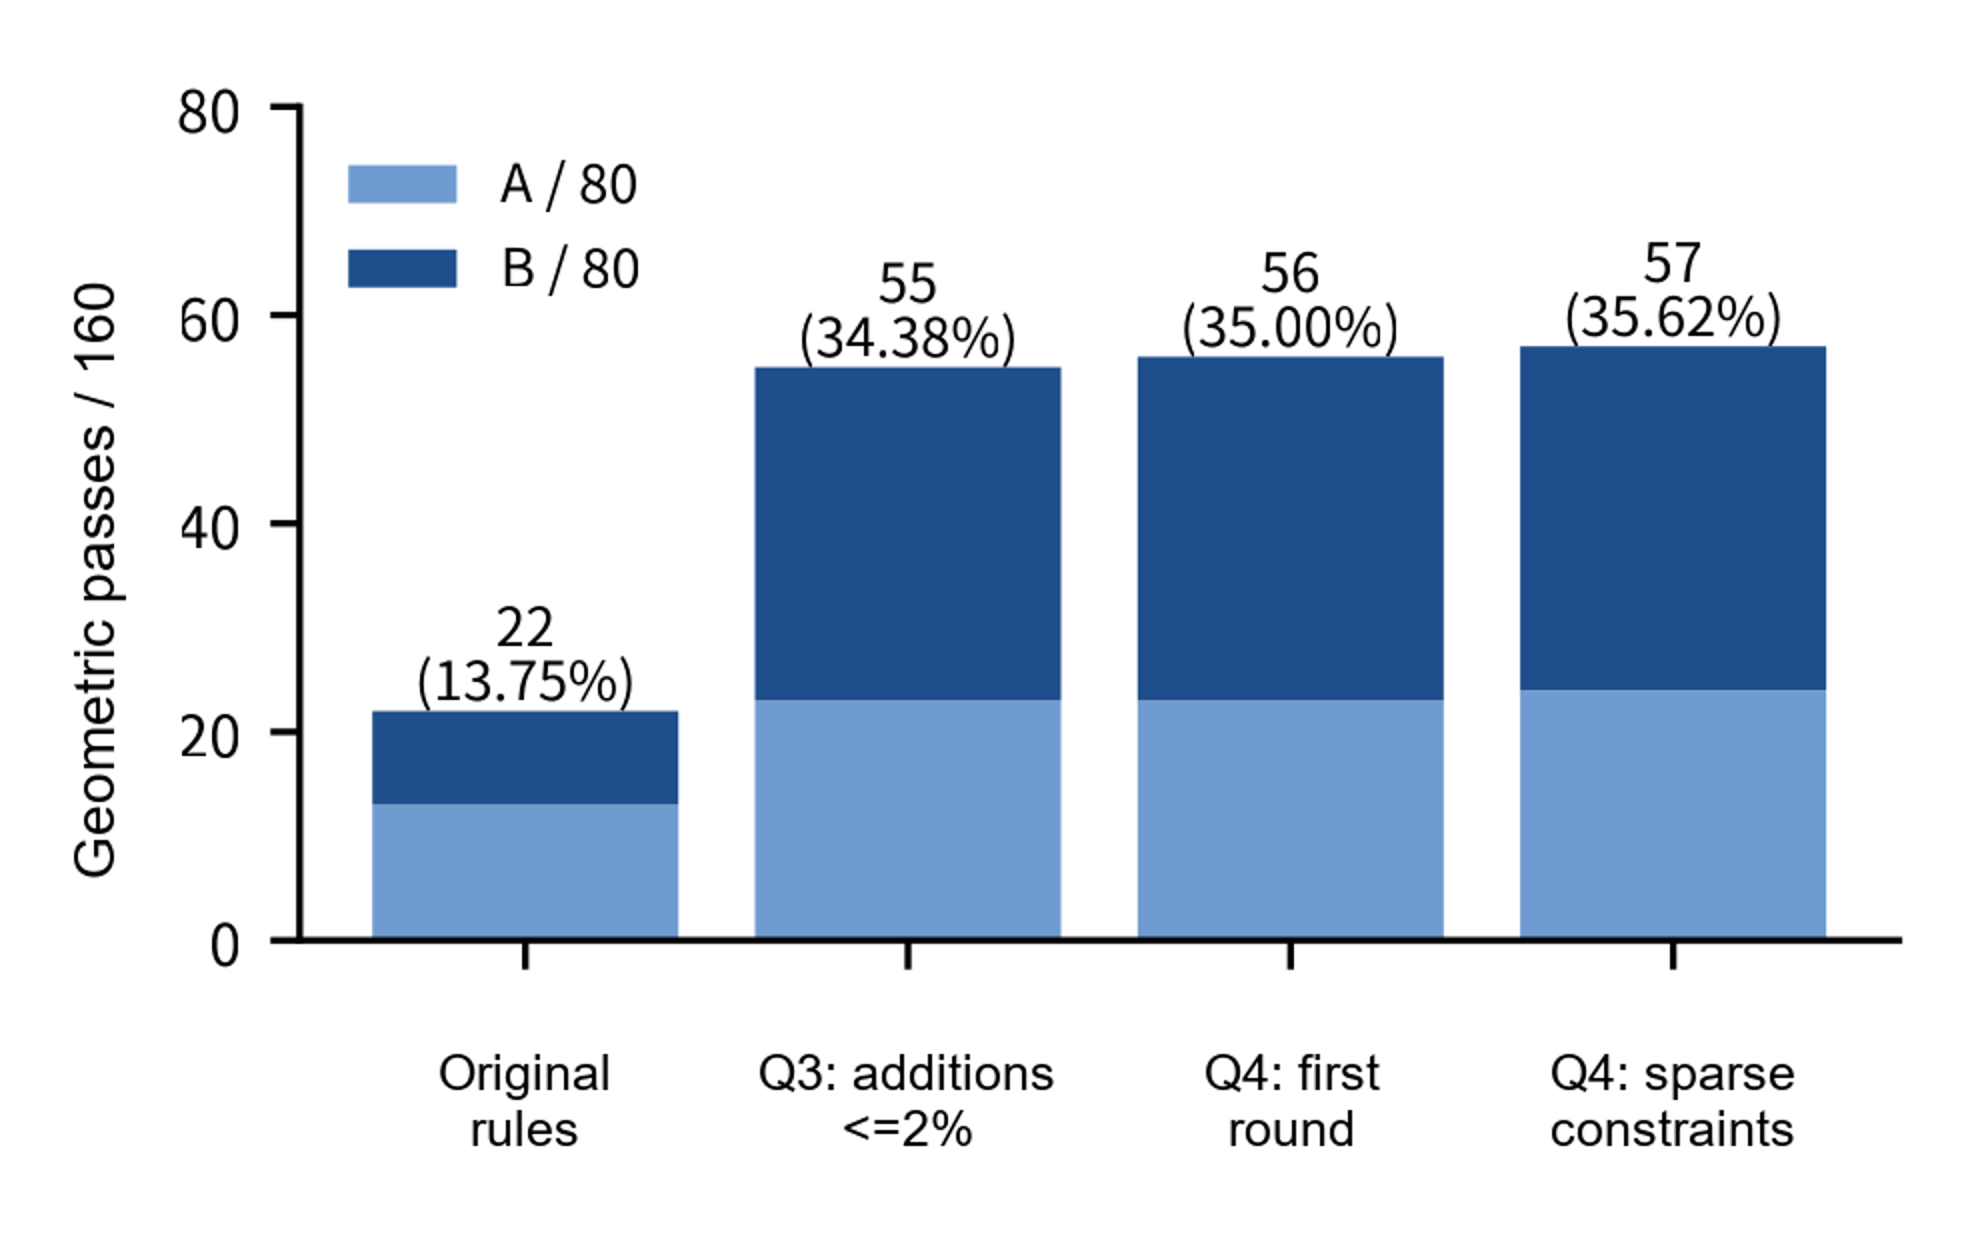
\includegraphics[width=0.72\textwidth]{figures/image16_en.png}
\caption{Historical results on a uniform 160-model sample. Version and numerical labels require verification.}
\end{figure*}

\begin{figure*}[!htbp]
\centering
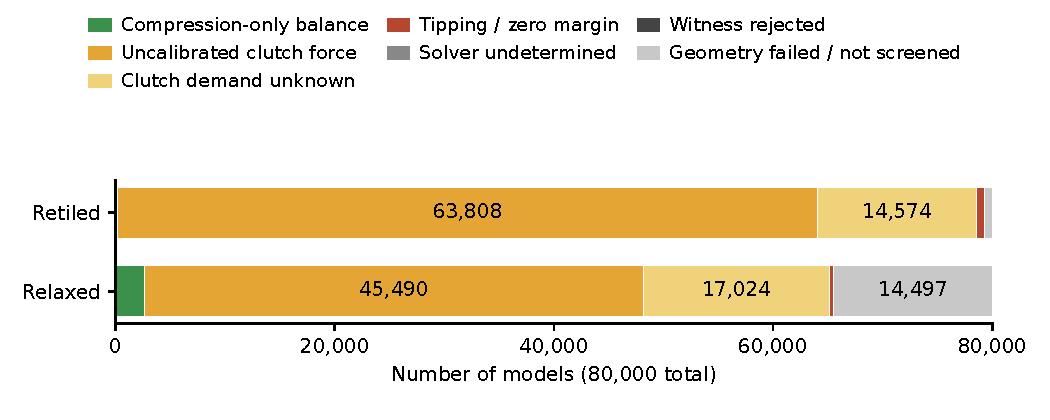
\includegraphics[width=\textwidth]{figures/image17_en.pdf}
\caption{Historical distributions of physical screening statuses; values as in the corresponding release reports. Counts refer to the specific releases shown and are kept separate from geometric pass rates.}
\end{figure*}


\section{Technical Appendix: Training Details}
\label{app:training}
Aggregate throughput is 24,448 tokens/s over eight GPUs, and the mean training loss is 0.0273. Evaluation and checkpointing run every 500 steps. With TRL~0.15, the unpacked multi-GPU path hangs after the first backward pass, which is why the TRL~0.17 stack is pinned. Because validation loss is lowest during epoch 2, two epochs would be a more economical setting for future runs (about one third less compute). The full software stack is transformers 4.51.3, trl 0.17.0, peft 0.15.2, datasets 3.6.0, and accelerate 1.6.0, with bf16 precision, gradient checkpointing, and unpacked sequences.

\begin{table}[!htbp]
\centering
\small
\begin{tabular}{lrr}
\toprule
Progress & Step & Validation loss \\
\midrule
Start & 500 & 0.1410 \\
--- & 1,500 & 0.0950 \\
--- & 10,500 & 0.0509 \\
--- & 22,500 & 0.0404 \\
$\approx$ End of epoch 1 & 44,500 & 0.0337 \\
--- & 65,500 & 0.0316 \\
Best (epoch 1.77) & 79,000 & 0.0308 \\
End of epoch 3 & 133,860 & 0.0339 \\
\bottomrule
\end{tabular}
\caption{Validation loss on the 2,000-sample validation subset. One epoch is $\approx$44,620 steps; the nearest evaluation to the end of epoch 1 is step 44,500.}
\label{tab:eval-loss}
\end{table}

% BrickGPT-paper column verified against arXiv:2505.05469 (Sec. 5.1 and Appendix A training details).
\begin{table*}[!htbp]
\centering
\small
\setlength{\tabcolsep}{5pt}
\begin{tabular}{lcc}
\toprule
Dimension & BrickGPT paper & Official Qwen3 script (ours) \\
\midrule
Base model & LLaMA-3.2-1B-Instruct & Qwen3-1.7B \\
LoRA & $r=32$, $\alpha=16$, dropout $0.05$, $q$/$v$ only (3.4M params) & $r=16$, $\alpha=32$, all linear layers \\
Learning rate & $2{\times}10^{-3}$ (AdamW) & $10^{-4}$ \\
Effective batch & 64 & 8 \\
Max length & 4,096 & 8,192 \\
Epochs & 3 & 3 \\
Hardware & 8$\times$RTX A6000, 12\,h & 8$\times$4090D, 25.3\,h \\
Data & StableText2Brick, 47k structures / 240k prompts & BrickMore-48, 79.3k models / 396,610 samples \\
\bottomrule
\end{tabular}
\caption{Our configuration versus the original BrickGPT paper \cite{brickgpt}. BrickGPT-paper values are taken from Sec.~5.1 and Appendix~A of arXiv:2505.05469 (base model, LoRA $r{=}32$, $\alpha{=}16$, dropout $0.05$, $q$/$v$ only with 3.4M parameters, AdamW learning rate $0.002$, global batch 64, 4096-token length filter, 3 epochs, 8$\times$RTX A6000 and 12\,h, and 47k+ structures / 240k prompts). The data organization, instruction template, absence of thinking mode, and LoRA paradigm follow BrickGPT; concrete hyperparameters follow the official Qwen3 adaptation, with the budget adjusted for the larger world, library, and corpus.}
\label{tab:brickgpt-recipe}
\end{table*}


\section{Technical Appendix: Additional Evaluation Material}
\label{app:eval}

\paragraph{November 16 evaluation.}
The run processed 1,315 exports and 10,520 images, with all four metrics present for each export. Group B contains 265 raw BrickForma Q8\_0 exports, 265 BrickGPT exports, and 265 BrickNet exports. The BrickGPT records report a $20^3$ world, seed 42, an eight-regeneration budget, and Gurobi disabled. Group A supplies only BrickGPT and BrickNet, with 260 exports per system (Table~\ref{tab:group-a}). The Group A BrickGPT run used the official merged checkpoint, a $20^3$ world, seed 42, and a 100-regeneration budget. Baseline means are reported within each cohort because the prompts and BrickGPT settings differ.
\begin{table}[t]
\centering\small
\setlength{\tabcolsep}{3pt}
\begin{tabular}{lrrrr}
\toprule
System & $P_{\mathrm{inv}}\downarrow$ & VQAScore $\uparrow$ & PE $\uparrow$ & SigLIP2 $\uparrow$ \\
\midrule
BrickGPT & \textbf{0.00\%} & \textbf{0.0401} & \textbf{0.1422} & \textbf{0.0125} \\
BrickNet & 18.97\% & 0.0142 & 0.1201 & 0.0007 \\
\bottomrule
\end{tabular}
\caption{Group A means on 260 matched prompts. This cohort contains BrickGPT and BrickNet.}
\label{tab:group-a}
\end{table}


\paragraph{Paired tests and truncation.}
Table~\ref{tab:sig} compares Group B alignment scores by prompt. We use a two-sided exact sign test and a two-sided Wilcoxon signed-rank test with the normal approximation, excluding ties from each test. Holm correction is applied separately to the six comparisons within each test. The largest adjusted $p$ is $4.62{\times}10^{-5}$ (rounded up). PE truncates 59 of 265 prompts and SigLIP2 truncates 106. On the untruncated subsets, BrickForma / BrickGPT / BrickNet score 0.1519 / 0.1430 / 0.1116 on PE (206 prompts) and 0.0404 / 0.0179 / 0.0009 on SigLIP2 (159 prompts).
\begin{table}[t]
\centering\small
\setlength{\tabcolsep}{3pt}
\begin{tabular}{llrrr}
\toprule
Baseline & Metric & W/L/T & Sign $p_H$ & Wilc.\ $p_H$ \\
\midrule
BrickGPT & VQAScore & 188/77/0 & $2.1\times 10^{-11}$ & $3.0\times 10^{-8}$ \\
 & PE & 166/99/0 & $4.6\times 10^{-5}$ & $3.8\times 10^{-6}$ \\
 & SigLIP2 & 168/97/0 & $3.1\times 10^{-5}$ & $2.2\times 10^{-6}$ \\
BrickNet & VQAScore & 237/28/0 & $1.2\times 10^{-41}$ & $5.9\times 10^{-33}$ \\
 & PE & 209/56/0 & $3.1\times 10^{-21}$ & $3.0\times 10^{-25}$ \\
 & SigLIP2 & 207/57/1 & $1.4\times 10^{-20}$ & $8.1\times 10^{-24}$ \\
\bottomrule
\end{tabular}
\caption{Two-sided paired tests on Group B. W/L/T counts BrickForma wins, losses and ties. Each test uses Holm correction across six comparisons.}
\label{tab:sig}
\end{table}


\paragraph{Earlier 114-prompt comparison.} BrickGPT outputs were generated in its native $20^3$ world (seed 42), whereas BrickForma places bricks in a $48^3$ workspace, which partly explains the difference in part counts.
The systems differ in candidate selection, filtering, and post-processing.
On the BrickForma side, 45 of the 114 comparison outputs, together with their prompts, were chosen by human review as the best of six candidate phrasings in a category--level group; a winner was available in 79 of 105 groups, and 45 of those winners entered this comparison.
The remaining 69 outputs come from later fill-in, regeneration, colleague, and review rounds: 35 replaced a judged winner in 34 groups, and 34 filled 26 groups in which no candidate had been judged acceptable; together the 114 outputs cover all 105 groups.\footnote{The six candidates are the five new-batch phrasings and one first-batch phrasing documented in the evaluation-set README. Among the 69: \texttt{review\_59} 21, a colleague success set 16, second-round redo 12, third-round fill-in 7, colleague \texttt{nine\_ldr} 7, regeneration 5, and \texttt{car\_trials} 1, as recorded in the 11-07 delivery manifest. BrickGPT was then run once on each selected prompt (seed 42); BrickNet contributed one accepted sample per prompt (up to 30 attempts).}
The 114 outcomes comprised 110 retiled layouts and four raw layouts. The earlier BrickGPT records report an eight-regeneration budget and Gurobi disabled.

\paragraph{Sensitivity of the earlier comparison.}
With equal weighting over the 105 category--level groups, BrickForma scores 0.2347 / 0.1840 / 0.1257 and BrickGPT scores 0.1511 / 0.1459 / 0.0318 on VQAScore / PE / SigLIP2. After excluding prompts truncated by each encoder, PE is 0.1821 versus 0.1445 on 89 prompts and SigLIP2 is 0.1088 versus 0.0301 on 85 prompts. The PE and SigLIP2 text encoders read at most 72 and 64 tokens, respectively.

\paragraph{Diagnostic cohort.}
To probe what the fine-tuned model learns, we inspected 525 BrickForma generations from a diagnostic set (21 categories $\times$ five levels $\times$ five phrasings). The 525-prompt diagnostic batch, together with 105 first-batch prompts, formed the six-phrasing candidate pool from which 45 of the 114 comparison outputs were selected (35 of them from the 525), as described above. Generation used seeds 42, 104, and 2026 in that order, moving to the next seed when a draft was incomplete or failed the geometry validator, then applied the 12--60--180\,s MILP ladder (the default loop of Algorithm~\ref{alg:inference-retiling}); raw drafts that already formed a single stud-connected component were kept unchanged. For 28 prompts a recovery path sampled seeds outside $S$; for two further prompts the solver budget was extended to 600\,s. Only 46 raw layouts (8.8\%) form a single stud-connected component without retiling; this rate shows no clear trend across levels (13, 9, 9, 7, and 8 for L1--L5) but varies strongly by category (e.g., 8/25 for sofa, 0/25 for basket and camera). All 479 failing raw layouts split into at least two stud components (median 5, maximum 33). Overlaps are a minor cause: 50 failing layouts contain duplicated voxels, 41 of them with at most five (median 2), and 429 contain none. The 2,240 detached fragments are mostly not grounded (1,320 airborne versus 920 grounded). The learned representation thus places bricks whose in-bounds voxel union is retained by retiling but that often fail to interlock across layers; all 525 final assemblies form a single stud-connected component with that union unchanged (Table~\ref{tab:diag} in Appendix~\ref{app:eval}). These checks evaluate stud connectivity and in-bounds voxel-union consistency, not prompt-level shape fidelity or spatial reasoning.

\begin{figure*}[t]
\centering
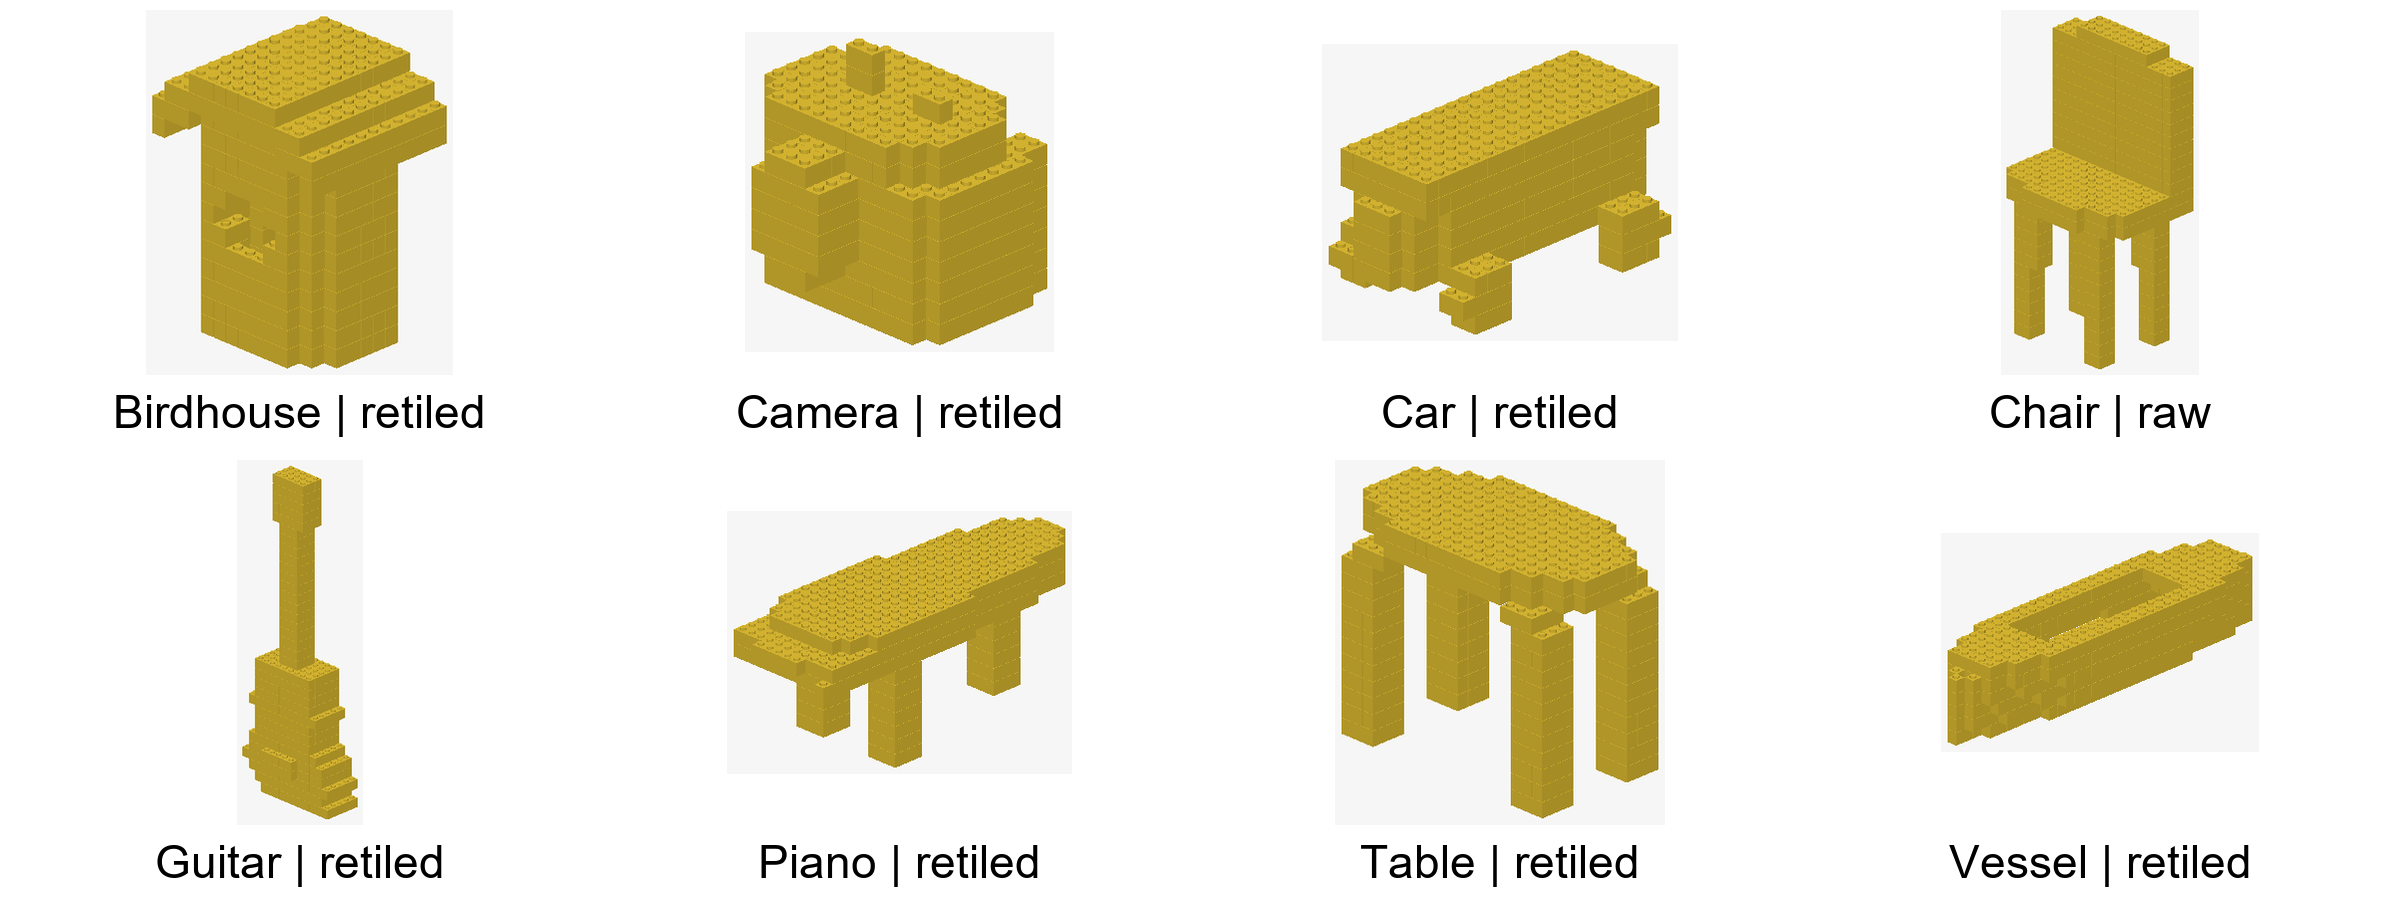
\includegraphics[width=\textwidth]{figures/generated_gallery_en.png}
\caption{BrickForma outputs from the earlier 114-prompt comparison. The chair is raw and the remaining examples are retiled.}
\end{figure*}


\begin{table*}[!htbp]
\centering
\small
\setlength{\tabcolsep}{3pt}
\begin{tabular}{lr}
\toprule
Quantity (525 prompts) & Value \\
\midrule
Raw layout is a single stud component & 46 (8.8\%) \\
Stud components per failing raw (med./max) & 5 / 33 \\
Failing raw layouts with duplicated voxels & 50 / 479 \\
Detached fragments (airborne / grounded) & 1,320 / 920 \\
MILP tier reached (12 / 60 / 180 / 600\,s) & 326 / 133 / 18 / 2 \\
Prompts resampled outside $S$ & 28 \\
Final: single stud comp., union unchanged & 525 / 525 \\
Raw bricks, median (range) & 183 (77--623) \\
Final assembly bricks, median & 452 \\
\bottomrule
\end{tabular}
\caption{Structural diagnostics of raw outputs (Section~\ref{sec:diagnostics}). ``Union unchanged'' means the final assembly covers exactly the in-bounds voxel union of the raw draft; it does not assess whether the shape matches the prompt.}
\label{tab:diag}
\end{table*}



\begin{figure*}[!htbp]
\centering
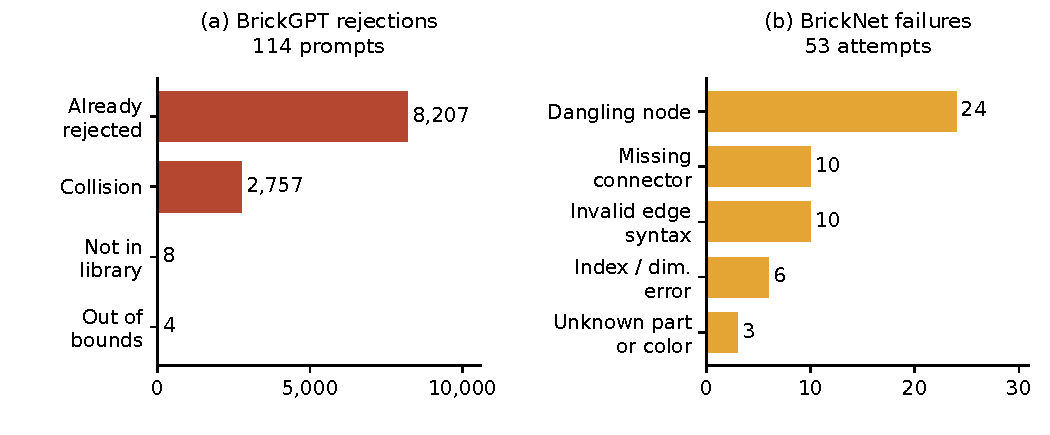
\includegraphics[width=\textwidth]{figures/image19_en.pdf}
\caption{Historical failure categories in the supplied reference; values as in the corresponding run records.}
\end{figure*}

\begin{figure*}[!htbp]
\centering
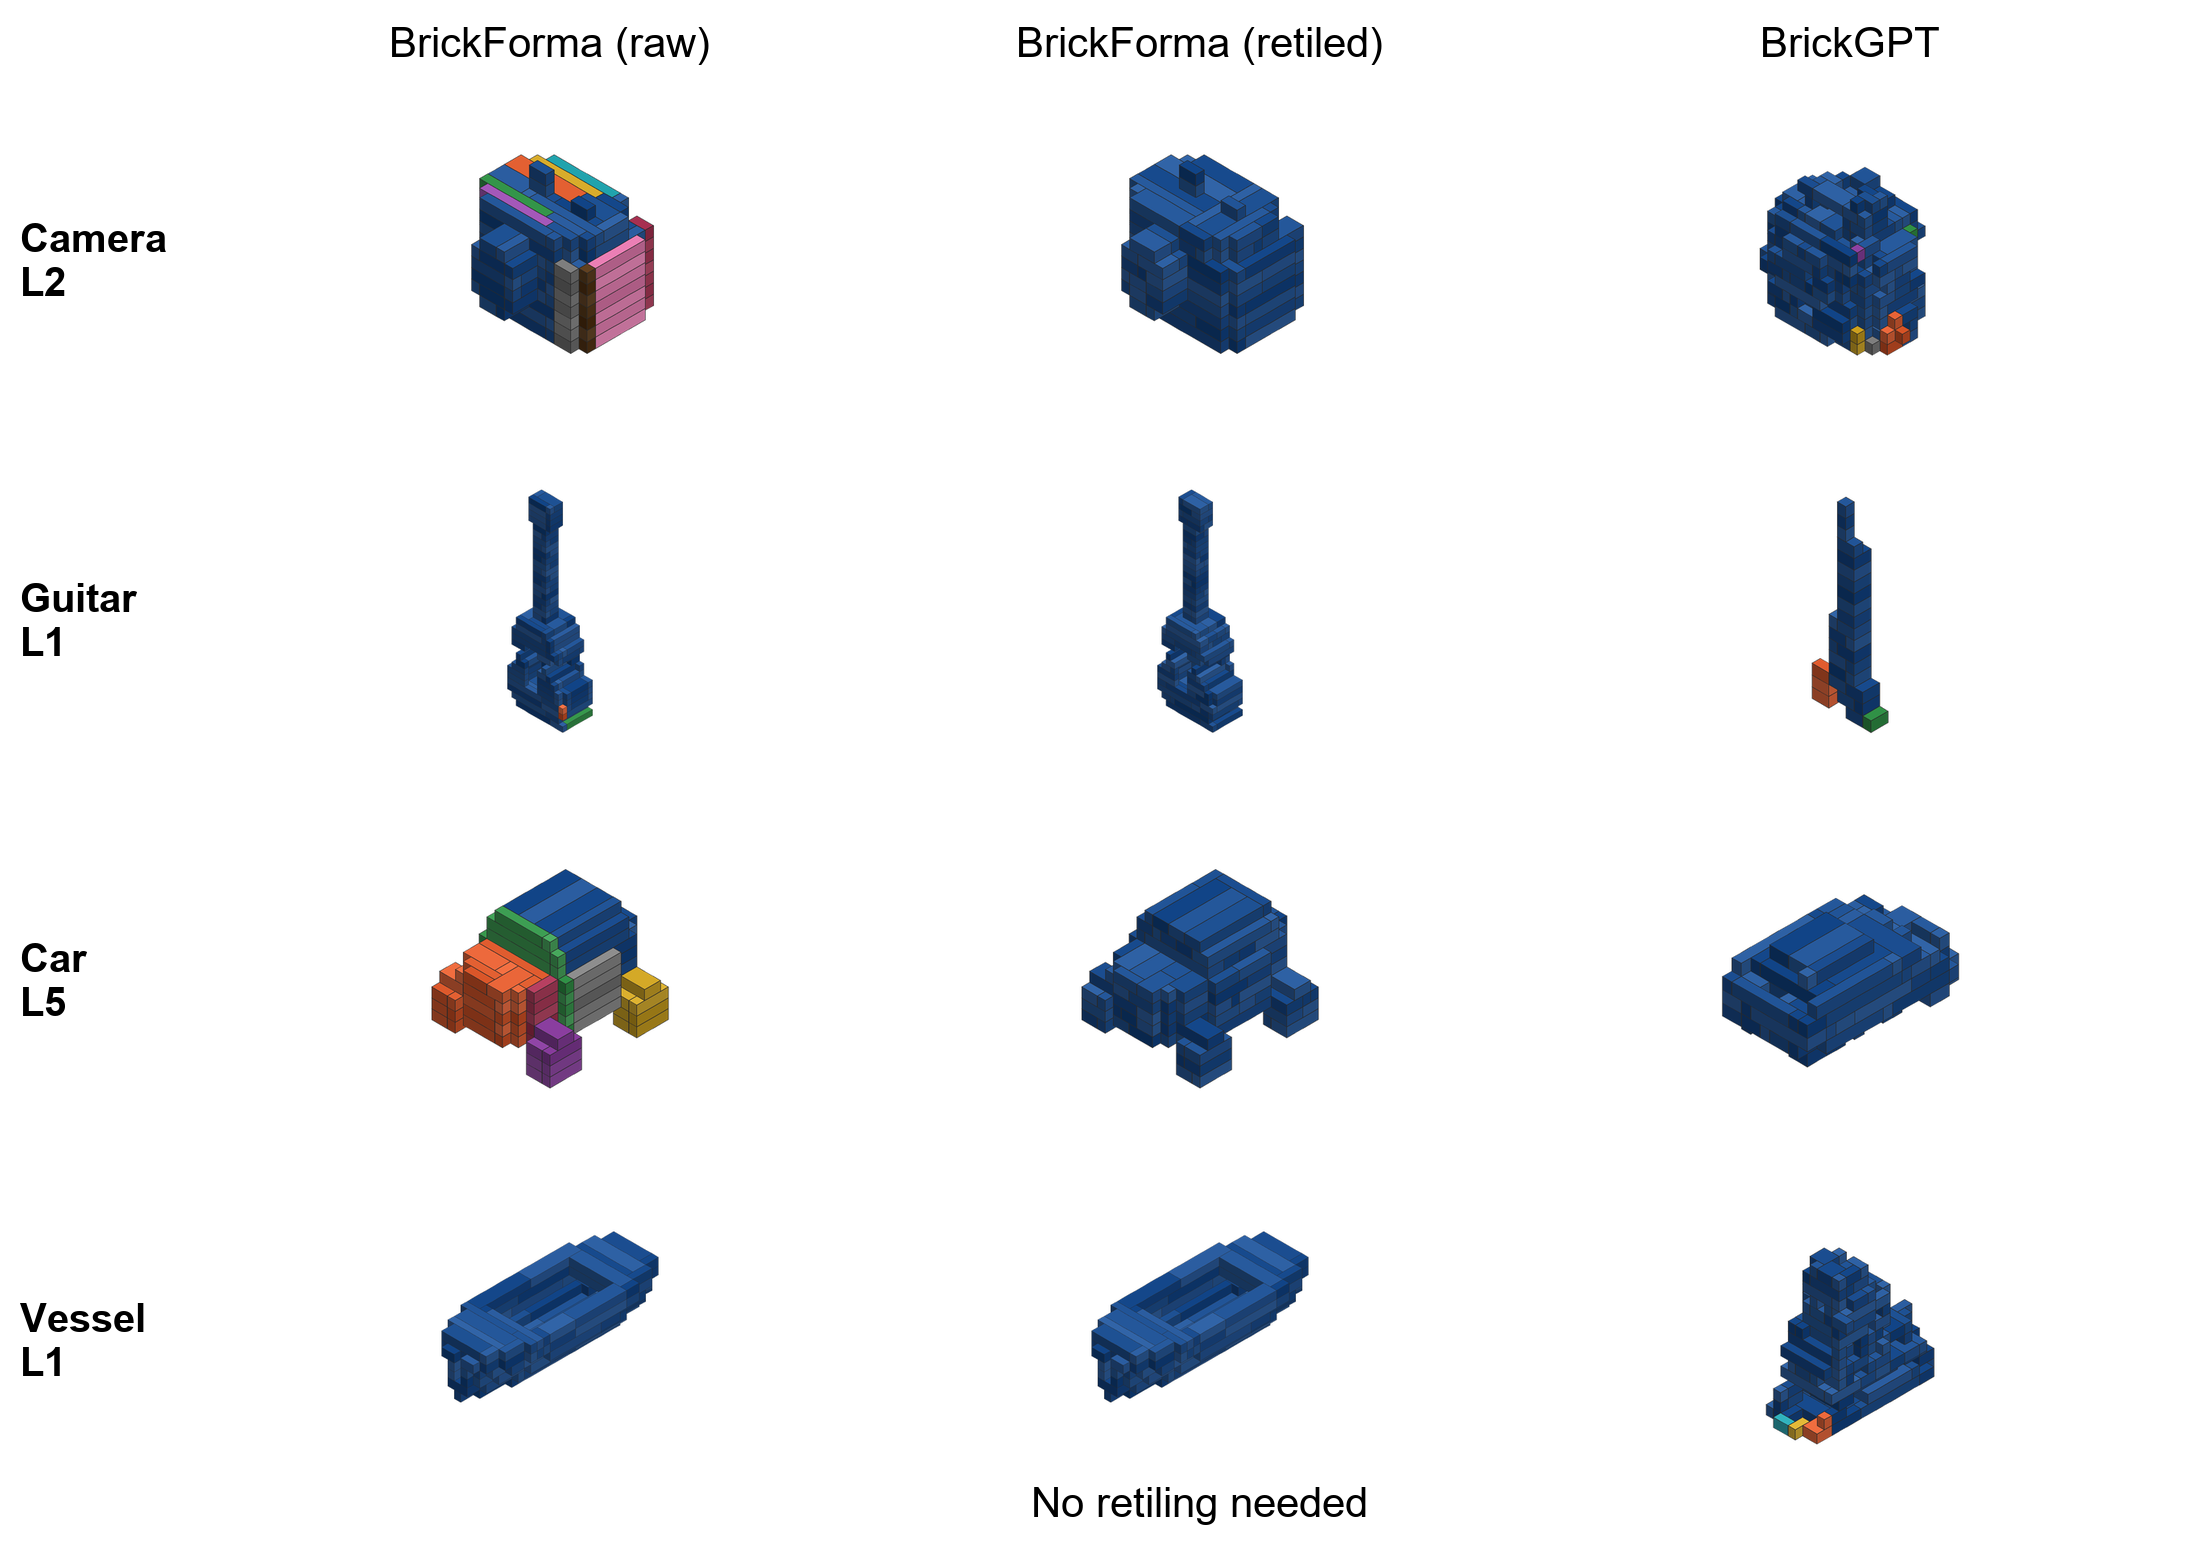
\includegraphics[width=\textwidth]{figures/original_comparison_en.png}
\caption{Qualitative historical examples from the supplied reference. Columns show raw and retiled outputs of our system and BrickGPT outputs.}
\end{figure*}

\begin{figure*}[t]
\centering
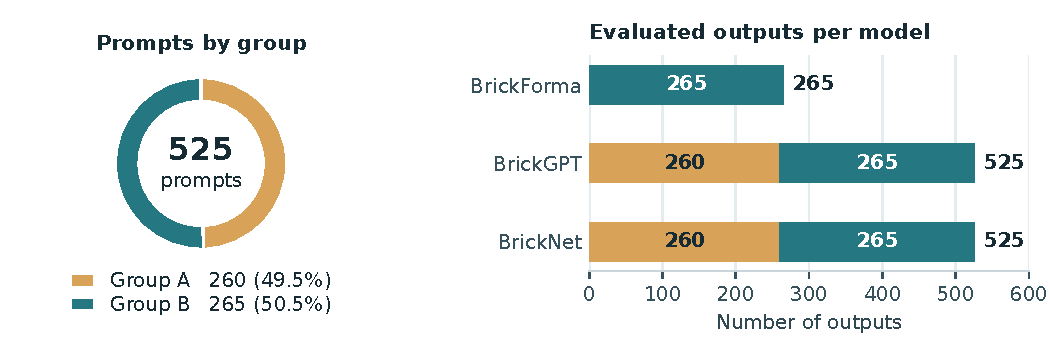
\includegraphics[width=\textwidth]{figures/comparison_20261116/01-cohorts.pdf}
\caption{Composition of the November 16 evaluation. Group A contains 260 shared prompts for BrickGPT and BrickNet. Group B contains 265 shared prompts for all three systems. The evaluation covers 525 distinct prompts and 1,315 exports.}
\label{fig:comparison-cohorts}
\end{figure*}

\begin{figure*}[t]
\centering
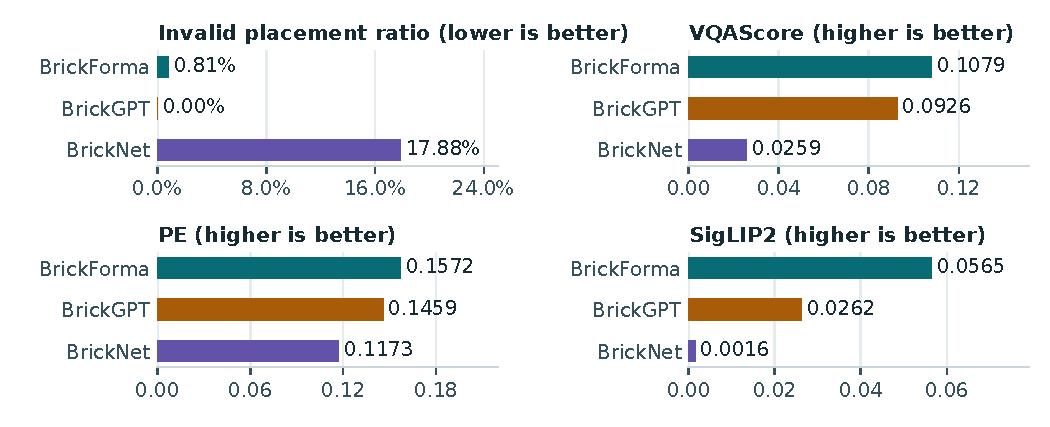
\includegraphics[width=\textwidth]{figures/comparison_20261116/02-means.pdf}
\caption{Mean scores on the 265 Group B prompts. Each mean assigns equal weight to each prompt. The plotted values correspond to Table~\ref{tab:main}.}
\label{fig:comparison-means}
\end{figure*}

\begin{figure*}[t]
\centering
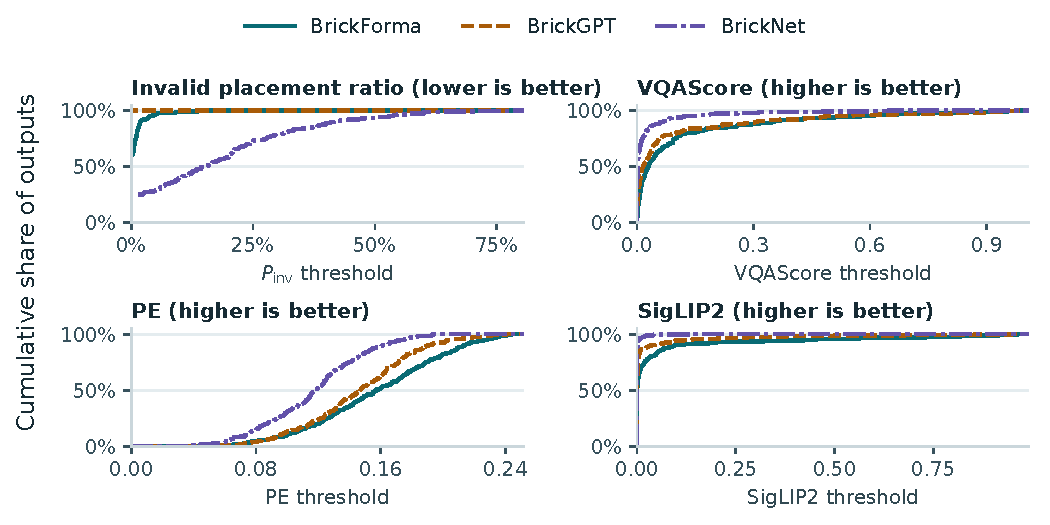
\includegraphics[width=\textwidth]{figures/comparison_20261116/03-distributions.pdf}
\caption{Empirical cumulative distributions of the four Group B scores. Each curve gives the fraction of a system's 265 outputs at or below the threshold on the horizontal axis.}
\label{fig:comparison-distributions}
\end{figure*}

\begin{figure*}[t]
\centering
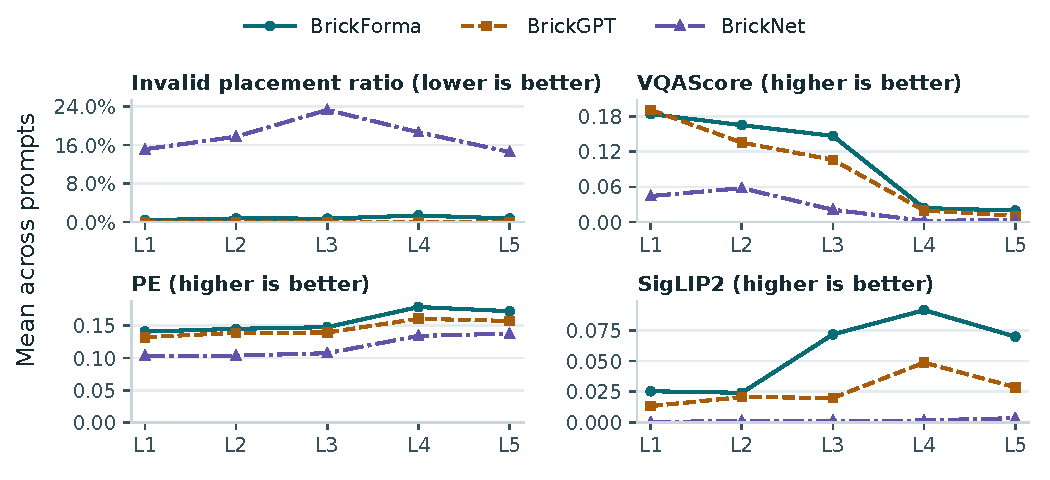
\includegraphics[width=\textwidth]{figures/comparison_20261116/04-by-level.pdf}
\caption{Group B mean scores by description level. Each point averages 53 prompts shared by all three systems. The plotted values correspond to Table~\ref{tab:levels}.}
\label{fig:comparison-levels}
\end{figure*}


\section{Technical Appendix: Historical Tables}
\label{app:historical}
The following transcribed tables preserve the historical reference material. They use different versions or evaluation criteria and are not substitutes for the current main comparison. Where a value is superseded by a verified number in the main text (e.g., Table~\ref{tab:training-data} and Appendix~\ref{app:dataset}), the main text takes precedence. Dashes indicate missing entries in the supplied source.
\begin{table*}[!htbp]\centering\small
\begin{tabular}{lr}\toprule
Item & Historical value \\ \midrule
Voxel models & 80,000 (40,000 per batch) \\
Categories / structural families & 21 / 40 per category \\
Grid / voxel count & $48^3$ / 750--1,250 \\
Prompt records & 400,000 (five bilingual records per model) \\
Uniqueness & 80,000 unique; 0 A/B duplicates \\
Overlap with historical hashes & 0 / 55,255 \\
Retile geometry passes & 79,298 (99.12\%) \\
Bricks in full preview & 12,718,389 \\
Final gravity equilibrium passes & 220 \\
Final and layer-prefix passes & 128 \\
\bottomrule\end{tabular}
\caption{Historical dataset statistics transcribed from the supplied reference. The geometry count refers to the old retile release, not the later integrated count. Verify the preview and physical-screening totals against version-matched reports.}
\end{table*}

\begin{table*}[!htbp]\centering\small
\setlength{\tabcolsep}{3pt}
\begin{tabular}{@{}l>{\raggedright\arraybackslash}p{3.9cm}>{\raggedright\arraybackslash}p{2.5cm}rrrr@{}}\toprule
Version & Connectivity & Voxel changes & Passes & Rate & Final & Both \\ \midrule
Strict v3 & Single; support $\geq$10\%, overhang $\leq$2 & None & 7,902 & 9.88\% & -- & -- \\
Relaxed & Each component grounded & +428,278 / -38,230 & 65,503 & 81.88\% & 2,650 & 478 \\
Retile & Each component grounded & +228,582 / -125 & 79,298 & 99.12\% & 220 & 128 \\
\midrule
\multicolumn{7}{l}{Uniform 160-model sample (seed 38177); not full-dataset results} \\
Baseline & Single stud-connected component & None & 22 & 13.75\% & -- & -- \\
Q3 & Single stud-connected component & Added $\leq$2\% & 55 & 34.38\% & 8 & 2 \\
Q4 (sparse) & Single stud-connected component & Added + removed $\leq$2\% & 57 & 35.63\% & 8 & 2 \\
\bottomrule\end{tabular}
\caption{Historical conversion-strategy table from the reference. Full-dataset and 160-model sample rows use different scopes; connectivity rules also differ. Final and Both columns report final-equilibrium and final-plus-prefix screening passes under the stated historical assumptions.}
\end{table*}

\begin{table*}[!htbp]\centering\small
\begin{tabular}{lrrr}\toprule
Item & BrickGPT & BrickNet 1.7B & BrickMore-48 \\ \midrule
Representation & $20^3$ bricks & Assembly graph & $48^3$ bricks \\
Criterion & stable & Parseable & -- \\
Passes & 66/114 & 114/114 & -- \\
Median parts & 126.5 & 22 & -- \\
Range & 19--497 & 6--48 & -- \\
Mean time (s) & 189.6 & -- & -- \\
\bottomrule\end{tabular}
\caption{Historical baseline table in the source reference. These criteria differ, and missing BrickMore-48 entries were marked TODO. This is not the current matched four-metric main table.}
\end{table*}

\begin{table*}[!htbp]\centering\small
\begin{tabular}{lrrrrl}\toprule
Level & $n$ & BrickGPT stable & GPT median bricks & Net median parts & BrickMore-48 \\ \midrule
L1 & 21 & 13 & 112 & 15 & -- \\
L2 & 21 & 15 & 118 & 22 & -- \\
L3 & 23 & 12 & 102 & 22 & -- \\
L4 & 25 & 12 & 140 & 21 & -- \\
L5 & 24 & 14 & 150.5 & 29.5 & -- \\
\bottomrule\end{tabular}
\caption{Historical level-wise baseline table transcribed from the reference. The original BrickMore-48 column was incomplete, and the other columns use different criteria.}
\end{table*}

\begin{table*}[!htbp]\centering\small
\begin{tabular}{lrrrr}\toprule
Method and source & $P_{\mathrm{inv}}$ & VQA & PE & SigLIP2 \\ \midrule
BrickGPT (literature, as transcribed) & 0.063 & 0.050 & 0.157 & 0.052 \\
BrickNet 1.7B (literature, as transcribed) & 0.260 & 0.593 & 0.282 & 0.631 \\
BrickGPT (114 prompts, historical placeholder) & -- & -- & -- & -- \\
BrickNet (114 prompts, historical placeholder) & -- & -- & -- & -- \\
BrickMore-48 (114 prompts, historical placeholder) & -- & -- & -- & -- \\
\bottomrule\end{tabular}
\caption{Original reference table with literature values and historical placeholders. Literature values use another evaluation set and must not be directly compared with the current Group B results; the precise $P_{\mathrm{inv}}$ definition and direction require checking against the original publication.}
\end{table*}



\end{document}
